%-----------------------------%
\selectlanguage{english}
\chapter{Scapegoat: Spotting the Faulty Component in Reconfigurable Software Systems}
\label{chp:scapegoat}
\markboth{Scapegoat: Spotting the Faulty Component in Reconfigurable Software Systems}{Chapter5}
%-----------------------------%

\coolphrase {
	\textbf{(\emph{Snot's} dead body lay down on the ground)} \\
	\vspace{1 mm}
	
	\emph{Witness} - And like every time, \emph{Snot}, he would fade a few shooters,\\
				     you know. Play it out until the pot's deep. Then he\hspace*{7 mm} \\
				     would snatch and run, you see what I'm saying?\hspace*{12 mm} 
	\vspace{1 mm}
	
	\emph{McNulty} - Every time?\hspace*{73 mm} 
	\vspace{1 mm}
	
	\emph{Witness} - Couldn't help himself.\hspace*{57 mm} 
	\vspace{1 mm}
	
	\emph{McNulty} - [\dots] You let him do this?\hspace*{50 mm} 
	\vspace{1 mm}
	
	\emph{Witness} - Naw man. We catch him and kick his [\dots]\hspace*{22 mm} 
	\vspace{1 mm}
	
	\emph{McNulty} - I got to ask you [\dots] -- if he did that every time -- why\hspace*{3 mm} \\
				   did you even let him into the games?\hspace*{32 mm} 
	\vspace{1 mm}
	
	\emph{Witness} - Huh?\hspace*{85 mm} 
	\vspace{1 mm}
	
	\emph{McNulty} - If \emph{Snot} always stole the money, why did you let him\hspace*{7 mm} \\
					 play?\hspace*{84 mm} 
	\vspace{1 mm}
	
	\textbf{(\emph{Witness} looks at \emph{McNulty} like he's an idiot)}
	\vspace{1 mm}
	
	\emph{Witness} - Got to \textbf{(pause)} this America, man.\hspace*{36 mm} 
}{The Wire, Season 1, Episode 1}


%Modern component frameworks support continuous deployment and simultaneous execution of multiple software components on
%top of the same virtual machine.
%However, isolation between the various components is limited.
%A faulty version of any one of the software components can compromise the whole system by consuming all available resources.
%In this paper, we address the problem of efficiently identifying faulty software components running simultaneously in a single virtual machine.
%Current solutions that perform permanent and extensive monitoring to detect anomalies induce high overhead on the system,
%and can, by themselves, make the system unstable.
%In this paper we present an optimistic adaptive monitoring system to determine the faulty components of an application.
%Suspected components are finely analyzed by the monitoring system, but only when required.
%Unsuspected components are left untouched and execute normally.
%Thus, we perform localized \textit{just-in-time} monitoring that decreases the accumulated overhead of the monitoring system.
%We evaluate our approach on two case studies against a state-of-the-art monitoring system and show that our technique correctly
%detects faulty components, while reducing overhead by an average of 92.98\%.


%\section{Introduction}\label{sec:intro}

%Modern computing systems, such as home automation, pervasive and ubiquitous systems are becoming a larger part of our lives.
%The tight connection with our living environment introduces new needs for these systems, such as the co-evolution of the system with its environment, the adaptation of the system to available resources and to users' behaviours, and the reliability of the system in front of faulty or malicious behaviours.
%Modern component frameworks assist software developers in coping with these new needs by providing introspection, reconfiguration, advanced technical services, among other facilities.
%These frameworks provide extensible middleware and assist developpers in managing technical issues such as security, transaction management, or distributed computing.
%They also support the simultaneous execution of multiple software components on the same virtual machine \cite{OSGI:r5,Kevoree,bruneton06}.
%% layer based ?
%
%While component frameworks simplify the programming model for software developers, the isolation between the various components is limited because they are collocated on the same virtual machine.
%This allows components to communicate efficiently and to share references to complex objects, something which is generally not possible when crossing the process boundary.
%However, one faulty software artifact may compromise the whole system by, for example, consuming all available resources on the machine.
%Furthermore, because these systems evolve in open environments where humans have central roles, software developers are unable to anticipate all future configurations of the application  at design-time \cite{baresi2006toward}.
%In these highly unpredictable environments, detecting irregular behaviour and maintaining the system in a consistent state is an important concern that can be addressed through continuous monitoring.

State of the art monitoring systems \cite{FrenotS04,KregerHaroldWilliamson03,Binder200645} collect data about the internal state of applications at runtime, such as the time spent executing a component, the amount of I/O and memory used, and the number of calls to a component.
The overhead that these monitoring systems introduce into applications is high, which makes it unlikely for them to be used in production systems.
Results presented in \cite{Binder:2009:PPV:1464245.1464249} show that overhead due to fine-grain monitoring systems can be up to a factor of 4.3.
The experiments presented in this chapter show that overhead grows with the size of the monitored software.
Thus, overhead greatly limits the scalability and usage of monitoring systems.

In this chapter, we address excessive overhead in monitoring approaches by introducing an optimistic adaptive monitoring system - Scapegoat - that provides lightweight global monitoring under normal conditions, and precise and localized monitoring when problems are detected.
Although our approach reduces the accumulated amount of overhead in the system, it also introduces a delay in finding the source of a faulty behaviour.
Our objective is to provide an acceptable trade-off between the overhead and the delay to identify the source of faulty behaviour in the system.

Our optimistic adaptive monitoring system is based on the following principles:
\begin{itemize}
\leftskip -.2in % see comments below
%\parindent -4in % see comments below
 \item \textbf{Contract-based resource usage.}
The monitoring system follows component-based software engineering principles. 
Each component is augmented with a contract that specifies their expected or previously calculated resource usage~\cite{Beugnard774917}. 
The contracts specify how a component uses memory, I/O and CPU resources.
 \item \textbf{Localized just-in-time injection and activation of monitoring probes.} 
Under normal conditions our monitoring system performs a lightweight global monitoring of the system. 
When a problem is detected at the global level, our system activates local monitoring probes on specific components in order to identify the source of the faulty behaviour.
The probes are specifically synthesized according to the component's contract to limit their overhead.
Thus, only the required data are monitored (e.g., only memory usage is monitored when a memory problem is detected), and only when needed.
  \item \textbf{Heuristic-guided search of the problem source.} 
We use a heuristic to reduce the delay of locating a faulty component while maintaining an acceptable overhead.
This heuristic is used to inject and activate monitoring probes on the suspected components. 
However, overhead and latency in finding the faulty component are greatly impacted by the precision of the heuristic.
A heuristic that quickly locates faulty components will reduce both delays and the accumulated overhead of the monitoring system.
We propose using Models@run.time techniques in order to build an efficient heuristic.
\end{itemize}

The evaluation of our optimistic adaptive monitoring system shows that, in comparison to other state-of-the-art approaches, the overhead of the monitoring system is reduced by up to 92.98\%.
Regarding latency, our heuristic reduces the delay to identify the faulty component when changing from global, lightweight monitoring to localized, just-in-time monitoring.
We also present a use case to highlight the possibility of using Scapegoat on a real application, that shows how to automatically find buggy components on a scalable modular web application.

The remainder of this chapter is organized as follows.
Section~\ref{sec:scapegoat-motivaing-example} motivates our work through a case study which is used to validate the approach.
A brief description of Kevoree, a platform for distributed component-based software development, is presented in Section~\ref{sec:kevoree-intro}.
Section~\ref{sec:scapegoat-approach} provides an overview of the Scapegoat framework.
It highlights how the component contracts are specified, how monitoring probes are injected and activated on-demand, how the Scapegoat framework enables the definition of heuristics to detect faulty components without activating all the probes, and how we benefit from Models@run.time to build efficient heuristics.
Section~\ref{sec:evaluation} evaluates the approach through a comparison of detection precision and detection speed with other approaches.
Section~\ref{sec:WebStudy} presents a use case based on an online web application\footnote{\url{http://cloud.diversify-project.eu/}} that leverages software diversity for safety and security purposes.
Finally, Section~\ref{sec:conclusion} discusses the approach and presents the conclusions of this chapter.

\section{Background and motivating example}\label{sec:background}

%\subsection{Motivating example\label{sec:motivatingexample}}

%In this section we present a motivating example for the use of an optimistic adaptive monitoring process in the context of a real-time crisis management system in a fire department. 
During a dangerous event, many firefighters are present and need to collaborate to achieve common goals.
%In a situation where many firefighters are present and need to collaborate to handle a dangerous event, 
Firefighters have to coordinate among themselves and commanding officers need to have an accurate real-time view of the system.

The Daum project\footnote{\url{https://github.com/daumproject}} provides a software application that supports firefighters in these situations.
The application runs on devices with limited computational resources because it must be mobile and taken on-site.
%As the software have to be mobile to take it on site, it is running on devices with limited computation resources.
It provides numerous services for firefighters depending on their role in the crisis.
In this chapter, we focus on the two following roles:
\begin{itemize}
\leftskip -.2in
 \item A collaborative functionality that allows commanding officers to follow and edit tactical operations. The firefighters' equipment include communicating sensors that report on their current conditions.
 \item A drone control system which automatically launches a drone equipped with sensors and a camera to provide a different point-of-view on the current situation.
\end{itemize}

%\todo{I don't get this for example. It is not relate to the previous sentence.}For example, one service is related to firefighter information monitoring to know the location, activity and health status of each firefighter involved on the crisis but also to get some information on their environment (e.g. temperature, toxic gas). Another service is in charge of the management of victims. They must be redirected according to their needs.

As is common in many software applications, the firefighter application may have a potentially infinite number of configurations. These configurations depend on the number of firefighters involved, the type of crisis, the available devices and equipment, among other parameters. 
Thus, it is generally not possible to test all configurations to guarantee that the software will always function properly. 
Consequently, instead of testing all configurations, there is a need to monitor the software's execution to detect faulty behaviours and prevent system crashes. 
However, fine-grained monitoring of the application can have excessive overhead that makes it unsuitable with the application and the devices used in our example.
Thus, there is a need for an accurate monitoring system that can find faulty components while reducing overhead.

The Daum project has implemented the firefighter application using a Component Based Software Architecture.  The application makes extensive use of the Kevoree\footnote{\url{http://www.kevoree.org}\label{note:kevoree}} component model and runtime presented in chapter \ref{chap:abstractions_and_resource_management}.

% Using our adaptive monitoring solution, we are able to reduce the overhead of the monitoring process keeping enough well response time to find faulty behaviors.



\subsection{Kevoree}
Kevoree is an open-source dynamic component platform, which relies on Models@run.time~\cite{BlairBF09} to properly support the dynamic adaptation of distributed systems.
Our use case application and the implementation of the Scapegoat framework make extensive use of the Kevoree framework.
The following subsections detail the background on component-based software architecture, introduce the Models@run.time paradigm and give an overview of the Kevoree platform.

\subsubsection{Component-based software architecture}

Software architecture aims at reducing complexity through abstraction and separation of concerns by providing a common understanding of component, connector and configuration~\cite{xadl,Medvidovic:2000,VanOmmering-et-al-00}.
One of the benefits is that it facilitates the management of dynamic architectures, which becomes a primary concern in the Future Internet and Cyber-Physical Systems~\cite{DBLP:journals/ase/NittoGMPP08, Johnson:2015:CSM:2735960.2735979}.
Such systems demand techniques that let software react to changes by self-organizing its structure and self-adapting its behavior~\cite{PanzicaLaManna:2012:LDU:2304736.2304764, Johnson:2015:CSM:2735960.2735979, Zhang:2009:MVD:1509239.1509262}.
Many works~\cite{cbse-conference} have shown the benefits of using component-based approaches in such open-world environments~\cite{baresi2006toward, Caporuscio:2010:AIA:1985522.1985547, Perez-Palacin:2010:PAO:1712605.1712614}.

To satisfy the needs for adaptation, several component models provide solutions to dynamically reconfigure a software architecture through, for example, the deployment of new modules, the instantiation of new services, and the creation of new bindings between components~\cite{Porter:2014:RMC:2602458.2602471, Zheng:2014:RCC:2679601.2680405, Irmert:2008:RAS:1370018.1370036, Ghezzi:2010:QDD:2163764.2163774}. 
In practice, component-based (and/or service-based) platforms like Fractal~\cite{bruneton06}, OpenCOM~\cite{BlairCULJ04}, OSGi~\cite{OSGI:r5} or SCA~\cite{SEINTURIER:2011:INRIA-00567442:1} provide platform mechanisms to support dynamic architectures.

%As a result, component-based platforms offer a challenging playground for building adaptive monitoring framework as they raise a new challenge in easing the open-world paradigm and they can be an element of the solution. 

%In this context, traditional software development, based on the closed-world assumption that the  boundary between system and environment is known and unchanging does not work.


\subsubsection{Models@run.time}
Built on top of dynamic component frameworks, Models@run.time denote model-driven approaches that aim at taming the complexity of dynamic adaptation.
It basically pushes the idea of reflection~\cite{morin09a} one step further by considering the reflection-layer as a real model: ``something simpler, safer or cheaper than reality to avoid the complexity, danger and irreversibility of reality''.
In practice, component-based and service-based platforms offer reflection APIs that allow instrospecting the application (e.g., which components and bindings are currently in place in the system) and dynamic adaptation (e.g., changing the current components and bindings).
While some of these platforms offer rollback mechanisms to recover after an erroneous adaptation~\cite{leger2010reliable}, the purpose of Models@run.time is to prevent the system from actually enacting an erroneous adaptation. 
In other words, the ``model at runtime'' is a reflection model that can be decoupled from the application (for reasoning, validation, and simulation purposes) and then automatically resynchronized.
This model can not only manage the application's structural information (i.e., the architecture), but can also be populated with behavioural information from the specification or the runtime monitoring data.


\subsubsection{The Kevoree framework\label{sec:kevoree}}	
% Se proteger un peu plus sur Kevoree pour big node / placer plus de ref / comparaison ?
%Language

%\todo{THIS SECTION IS VERY UNCLEAR!!!}

Kevoree provides multiple concepts that are used to create a distributed application that allows dynamic adaptation. The \emph{Node} concept is used to model the infrastructure topology and the \emph{Group} concept is used to model the semantics of inter-node communication, particularly when synchronizing the reflection model among nodes. 
Kevoree includes a \emph{Channel} concept to allow for different communication semantics between remote \emph{Components} deployed on heterogeneous nodes. 
All Kevoree concepts (\textit{Component}, \textit{Channel}, \textit{Node}, \textit{Group}) obey the object type design pattern~\cite{johnson_type_1997} in order to separate deployment artifacts from running artifacts.  

%Platforms
Kevoree supports multiple execution platforms (e.g.,~Java, Android, MiniCloud, FreeBSD, Arduino). For each target platform it provides a specific runtime container. 
%Tools
Moreover, Kevoree comes with a set of tools for building dynamic applications (a graphical editor to visualize and edit configurations, a textual language to express reconfigurations, several checkers to valid configurations). 

%The remainder of this section describes the main concepts of the Kevoree component model that are useful to understand the scapegoat approach.
%\todo{One sentence to explicit how Kevoree and Model@Runtime help the development of our approach}

As a result, Kevoree provides a promising environment by facilitating the implementation of dynamically reconfigurable applications in the context of an open-world environment.
Because our goal is to design and implement an adaptive monitoring system, the introspection and the dynamic reconfiguration facilities offered by Kevoree suit the needs of the ScapeGoat framework.
%As a result, component-based platforms offer a challenging playground for building adaptive monitoring framework as they raise a new challenge in easing the open-world paradigm and they can be an element of the solution. 



%\subsection{Dynamic Adaptation with Kevoree}
%Kevoree aims at providing advanced adaptation capabilities to different types of nodes:
%\begin{itemize}
%\setlength{\itemsep}{0pt}
%\setlength{\parskip}{0pt}
%\setlength{\parsep}{0pt}
%\item 
%\noindent{\bf Level 1: Parametric adaptation.} Dynamic update of parameter values, e.g. change of sampling rate in a component that wraps a physical sensor (adaptation of instance properties).

%\item 
%\noindent{\bf Level 2: Architectural adaptation.} Dynamic addition or removal of bindings or components, e.g. replication of software components and channels on different nodes to perform load balancing (adaptation of instances graph).

%\item 
%\noindent{\bf Level 3: Dynamic provisioning of types.} Hot deployment of component types that were not foreseen before the initial deployment of the system. 
%This allows for system evolution by enabling parametric and architectural reconfigurations, including management of instances for types that are added and managed dynamically (adaptation of types).

%%\item 
%%\noindent{\bf Level 4: Adaptation for remote management.} Nodes supporting level~4 adaptation participate in a remote management layer, which supervises less powerful nodes. 
%%This layer monitors remote nodes by requesting their current Kevoree model;
%%the layer triggers dynamic adaptation of nodes by sending precomputed reconfiguration scripts to them. 
%%This remote adaptation process supports seamless management of less powerful nodes by a more powerful one, which has enough resources to build and evaluate new and appropriate  configurations.
%\end{itemize}

%The adaptation engine relies on a model comparison between two Kevoree models to compute a  script for a safe system reconfiguration; execution of this script brings the system from its current configuration to the new selected configuration~\cite{morin09a}. 
%Model comparison yields  a delta-model defining changes (using CRUD operations) that should be applied on the source model to obtain the target model. 
%Planification algorithms~\cite{daubert} use this delta-model as input in order to defined an efficient schedule of the adaptation steps. 
%The delta-model is finally compiled into a Kevoree script. 
%The Kevoree Script language (KevScript for short) is a core language for describing reconfiguration.
%KevScript  is comparable to FScript for Fractal Component Model~\cite{DBLP:journals/adt/DavidLLC09}. 
%Execution of a KevScript directly adapts a Kevoree system, without the need for  a full Kevoree model definition. 
%Such adaptation scripts are written by designers, or they can be generated  by automated processes ({\em e.g.} within a  control loop managing the Kevoree system).

%\hl{(Johann) What is the point of having so much detail about the Kevoree adaptation framework for this paper? It's not clear to me or we should have a last paragraph explaining a bit in what this is usefull for the rest of the paper.}

\section{The Scapegoat framework\label{sec:scapegoat-approach}}
%\section{Adaptive optimistic monitoring with the ScapeGoat framework\label{sec:approach}}

%\todo{Completely change this section !!! We need to make the link with the background here, and to provide a picture with an overview}

Our optimistic adaptive monitoring system extends the Kevoree platform with the following principles: i) component contracts that define per-component resource usage, ii) localized and just-in-time injection and activation of monitoring probes, iii) heuristic-guided faulty component detection. The following subsections present an overview of these three principles in action. 
%The monitored system follows the principles of component based software engineering.
%Each component is augmented with a contract that defines their expected resource usage.
%The contract specifies how the component is supposed to use, for example, memory, I/O and CPU resources.
 
%  \item \textbf{Localized and just-in-time injection and activation of monitoring probes.}
%Under normal conditions, our monitoring system performs lightweight global monitoring of the application.
%When a problem is detected at the global level, we activate local monitoring probes on components.
%Probes are synthesized according to the components' contracts to limit \hl{[capacity and?]} overhead.
%Thus, fine-grain monitoring is only applied when needed and only on the resource-data of interest.

% \item \textbf{Heuristic guided search of the problem source.} 
%To reduce latency and maintain an acceptable overhead, we use a heuristic to guess the locality of the faulty components.
%This heuristic is used to select where we inject and activate our monitoring probes.
%In short, it calculates suspected components.
%Our heuristic leverage the use of models@run.time by assigning a greater probability to recently updated components 
%\end{itemize}


\subsection{Specifying component contracts} \label{componentcontract}
%\assignedtodo{Inti}{Improve the contract as reviewer 3 suggested. (more relevant if using patterns based on the evolution of %values rather than maximum values)}

In Scapegoat, we follow the contract-aware component classification~\cite{Beugnard774917}, which applies B. Meyer's Design-by-Contract principles~\cite{Meyer:1992:ADC:618974.619797} to components.
%This framework proposes to apply B. Meyer's Design by Contract~\cite{Meyer:1992:ADC:618974.619797} principles to components with an attempt at generalization.
%ScapeGoat mainly introduces the fourth level of contract (\textit{Quality of Service}) in Kevoree in supporting the specification of instant worst case situation for memory consumption, CPU and Input/Output resource consumption and time period average for the same resources kinds. 
In fact, Scapegoat provides Kevoree with \textit{Quality of Service} contract extensions that specify the worst-case values of the resources the component uses.
The resources specified are memory, CPU, I/O and the time to service a request.
The exact semantic of a contract in Scapegoat is: \textit{the component will consume at most $X$ resource if it receives at most $N$ requests on its provided ports.}  
%The resources specified are memory, CPU, I/O and request throughput.  

For example, for a simple Web server component we can define a contract on the number of instructions per second it may execute \cite{Binder200645} and the maximum amount of memory it can consume.
The number of messages can be specified per component or per component-port.
In this way, the information can be used to tune the usage of the component roughly or detailedly.
An example is shown in Listing~\ref{contractspec}.\footnote{Examples of contract for the architecture presented in section~\ref{sec:scapegoat-motivaing-example} can be found at \url{http://goo.gl/uCZ2Mv}.} This contract extension follows the component interface principle~\cite{Henzinger03}, and allows us to detect if the problem comes from the component implementation or from a component interaction.
That is, we can distinguish between a component that is using excessive resources because it is faulty, or because other components are calling it excessively.


\lstset{frame=tb,
  aboveskip=3mm,
  belowskip=3mm,
  showstringspaces=false,
  columns=flexible,
  basicstyle=\color{black}\scriptsize,
  numbers=none,
  numberstyle=\color{gray}\scriptsize,
  keywordstyle=\color{blue}\scriptsize,
  commentstyle=\color{dkgreen}\scriptsize,
  stringstyle=\color{purple}\scriptsize,
  breaklines=true,
  breakatwhitespace=true,
  tabsize=2,,
  captionpos=b,
  language=java
}

\begin{lstlisting}[escapeinside={(*}{*)},caption=Component contract specification example,label=contractspec,float=!h]
add node0.WsServer650 : WsServer

//Specify that this component can use 2580323 CPU 
//instructions per second
set WsServer650.cpu_wall_time = 2580323 intr/sec 

//Specify that this component can consume a maximum of 15000
//bytes of memory
set WsServer650.memory_max_size = 15000 bytes

//Specify that the contract is guaranteed under the assumption that 
//we do not receive more than 10k messages on the component and 
//10k messages on the port named service
//(this component has only one port)
set WsServer650.throughput_all_ports = 10000 msg/sec
set WsServer650.throughput_ports.service = 10000 msg/sec

\end{lstlisting}

%They introduced a classification of contracts in four levels. 
%It can be summarized as:
%\begin{itemize}
%\item \textbf{Syntactic} (or basic) The goal is to make the system work. 
%It is generally specified with Interface Definition Languages (IDLs), as well as typed object-based or object-oriented languages.
%It ensures the components can be assembled.
%\item \textbf{Behavioral} The goal is to specify each operation. It is generally specified with a couple of assertions:
%a precondition and a postcondition. It ensures the operations offered and required are not only
%syntactically compatible but also semantically.
%\item \textbf{Synchronization} The goal is to specify the coordination of operations. It can be specified with an
%automaton labeled with operations. It ensures the operations are used in the proper order.
%\item \textbf{Quality of Service} The goal is to quantify a few features associated to operations. Performance, availability and quality of result can be specified and negotiated at that level.
%\end{itemize}

%Scapegoat approach is mainly built on top of Kevoree (section~\ref{sec:kevoree}). Kevoree supports only syntactic contracts between components. We introduce for Scapegoat a way \hl{to specify behavioural contracts, synchronization contract and quality of service contracts}\todo{Ok we propose something about "behavioural contracts with resource useage stuff but I'm not sure we propose something else...}. For synchronization and behavioral contract, we mainly reuse previous work~\cite{BaraisDuchien05} to provide a language for the specification of these contracts. To specify quality of services, Scapegoat introduces 
%
%As a basic example, a component \emph{A} can specify two ports with operations (level 1). 
%These operations can have pre and post conditions (level 2), the architect can provide a synchronization contract to specify that these ports cannot be accessed simultaneously (level 3) and that it can consume percent of CPU in a peak and an average of 10 percent of CPU resource per minute. \hl{SHOULD WE PROVIDE A REAL COMPONENT SPECIFICATION, SHOULD WE DISCUSS HOW WE infer these contract ?}
%\hl{(Johann) I think we should provide a real example here but not how we infered it}\todo{What are the levels ?}

\subsection{An adaptive monitoring framework within the container} \label{monitorContainer}

%In Scapegoat, the behavioral and synchronization contract correctness are not managed by the container.  To guarantee the behavioral component contracts, assertions are embedded at runtime within the component implementation, they can be activated on demand. In Kevoree, to guarantee concurrent access to ports, they are protected behind an actor model~\cite{Hewitt:1973:UMA:1624775.1624804,hewitt2010actor}. In the presence of a synchronization contracts between ports, an actor is generated before the actor of each port to manage the concurrent access to ports. This actor handles the reception of external messages corresponding to the service invocation request and dispatch the request to the service implementations.

Scapegoat provides a monitoring framework that adapts its overhead to current execution conditions and leverages the architectural information provided by Kevoree to guide the search for faulty components.
The monitoring mechanism is mainly injected within the component container. 

% an way to deal with an adaptive framework for quality of service (resource consumption) contracts. 
Each Kevoree node/container is in charge of managing the component's execution and adaptation.
Following the Models@run.time approach, each node can be sent a new architecture model that corresponds to a system evolution.
In this case, the node compares its current configuration with the configuration required by the new architectural model and computes the list of individual adaptations it must perform.
Among these adaptations, the node is in charge of downloading all the component packages and their dependencies, and loading them into memory.
During this process, Scapegoat provides the existing container with (i) checks to verify that the system has enough resources to manage the new component, (ii) instrumentation for the component's classes in order to add bytecode for the monitoring probes, and iii) communication with a native agent that provide information about heap utilization.
Scapegoat uses the components' contracts to check if the new configuration will not exceed the amount of resources available on the device.
It also instruments the components' bytecode to monitor object creation (to compute memory usage), to compute each statement (for calculating CPU usage), and to monitor calls to classes that wrap I/O access such as the network or file-system.
In addition, Scapegoat provides a mechanism to explore the Java heap and to account for memory consumption with an alternative mechanism.

We provide several instrumentation levels that vary in the information they obtain and in the degree they impact the application's performance:
\begin{itemize}
\leftskip -.2in
	\item \textbf{Global monitoring} does not instrument any components, it simply uses information provided directly by the JVM.
	\item \textbf{Memory instrumentation} or memory accounting, which monitors the components' memory usage.
	\item \textbf{Instruction instrumentation} or instruction accounting, which monitors the number of instructions executed by the components.
	\item \textbf{Memory and instruction instrumentation}, which monitors both memory usage and the number of instructions executed.	
\end{itemize}

Probes are synthesized according to the components' contracts.
For example, a component whose contract does not specify I/O usage will not be instrumented for I/O resource monitoring.
All probes can be dynamically activated or deactivated.
Note that due to a technical limitation, one of the two probes implemented to check memory consumption must be always activated.  
%with the exception of memory usage probes based on instrumenting the bytecode.
This memory consumption probes, based on bytecode instrumentation must, remain activated to guarantee that all memory usage is properly accounted for, from the component's creation to the component's destruction.
Indeed, deactivating this memory probes would cause object allocations to remain unaccounted for.
However, probes for CPU, I/O usage and the second probe for memory can be activated on-demand to check for component contract compliance.

%\todo{For Walter: Review this paragraph}
We propose two different mechanisms to deal with memory consumption.
The first mechanism is based on bytecode instrumentation and accounts for each object created. 
As mentioned previously, this mechanism cannot be disabled.
%The second mechanism is based on exploring the JVM heap on demand to capture the consumption just-in-time.
The second mechanism is a just-in-time exploration of the JVM heap, performed on demand.
%, to capture consumption.
These two mechanisms differ in i) when the computation to account for consumption is done, ii) how intensive it is, and iii) in the way the objects are accounted for.
Computations in the first mechanism are spread throughout the execution of the application, short and lightweight operations are executed every time a new object instance is created or destroyed.
Objects are always accounted to the component that creates them.
Computations in the second mechanism occur only on demand but are intensive because they involve traversing the graph of living objects in the heap.
The accounting policy follows the paradigm of assigning objects to the component that is holding them and, if an object is reachable from more than one component, it is accounted to either one randomly, as suggested in~\cite{Price:2003:GCM:829515.830545,dsn/09/geoffray/ijvm}; we call this second mechanism \textbf{Heap Exploration}.


%\todo{For Walter: Review this paragraph}
%todo: NEEDS WORK
%To take full advantage of having probes that may be dynamically activated and deactivated, 
We minimize the overhead of the monitoring system by activating selected probes only when a problem is detected at the global level.
We estimate the most likely faulty components and then activate the relevant monitoring probes.
Following this technique, we only activate fine-grain monitoring on components suspected of misbehavior.
After monitoring the subset of suspected components, 
if any of them are found to be the source of the problem, the monitoring system terminates.
%if any of them are indeed found to be faulty, the monitoring system terminates its job and determines that these components are the source of the problem.
However, if the subset of components is determined to be healthy, the system starts monitoring the next most likely faulty subset.
This occurs until the faulty component is found.
%If no components are found to be faulty and the problem still exists at the global level, the entire process is repeated.
If no components are found to be faulty, we fallback to global monitoring. If the problem still exists the entire process is restarted. This can occur in cases where, for example, the faulty behavior is transient or inconsistent.
The monitoring mechanism implemented in Scapegoat is summarized in Listing \ref{algo:monitoring}.

\lstset{frame=tb,
  aboveskip=3mm,
  belowskip=3mm,
  showstringspaces=false,
  columns=flexible,
  basicstyle=\color{black}\scriptsize,
  numberstyle=\color{gray}\scriptsize,
  keywordstyle=\color{blue}\scriptsize,
  commentstyle=\color{dkgreen}\scriptsize,
  stringstyle=\color{purple}\scriptsize,
  breaklines=true,
  breakatwhitespace=true,
  tabsize=2,
  captionpos=b,
  language=java,
  numbers=left,
  stepnumber=1,    
  firstnumber=1,
  numberfirstline=true
}

\begin{lstlisting}[escapeinside={(*}{*)},caption=The main monitoring loop implemented in Scapegoat,label=algo:monitoring,float=!h]
monitor(C: Set<Component>, heuristic : Set<Component>(*$\rightarrow$*)Set<Component>)
	init memory probes ((*${c \mid c \in C \wedge c.memory\_contract\ne\emptyset}$*))
	while container is running
		wait violation in global monitoring
		checked = (*$\emptyset$*)
		faulty = (*$\emptyset$*)
		while (*$ checked \ne C \wedge faulty = \emptyset$*)
			subsetToCheck = heuristic ( C (*$\setminus$*) checked )
			instrument for adding probes ( subsetToCheck )
			faulty = fine-grain monitoring( subsetToCheck )
			instrument for removing probes ( subsetToCheck )
			checked = checked (*$\cup$*) subsetToCheck
		if faulty (*$\ne \emptyset$*)
			adapt the system (faulty, C)

fine-grain monitoring( C : Set<Component> )
	wait few milliseconds // to obtain good information
	faulty = (*$ \{ c \mid c \in C \wedge c.consumption > c.contract \} $*)
	return faulty
\end{lstlisting}


As a result, we consider that applications are executing under the conditions of one of the following monitoring modes:
\begin{itemize}
\leftskip -.2in
	\item \textbf{No monitoring.} The software is executed without any monitoring probes or modifications.
	\item \textbf{Global monitoring.} Only global resource usage is being monitored, such as the CPU and memory usage at the Java Virtual Machine (JVM) level.
	\item \textbf{Full monitoring.} All components are being monitored for all types of resource usage. This is equivalent to current state-of-the-art approaches.
	\item \textbf{Localized monitoring.} Only a subset of the components are monitored.
	\item \textbf{Adaptive monitoring.} The monitoring system changes from Global monitoring to Full or Localized monitoring if a faulty behaviour is detected.
%	\item When we are using adaptive monitoring and the heuristic we are using is $h(C) = C$ we call this \textbf{All Components} strategy.
\end{itemize}
For the rest of this chapter we use the term \textbf{all components} for the adaptive monitoring policy that indicates that the system changes from \emph{global monitoring} mode to \emph{full monitoring} mode if and when a faulty behaviour is detected.

%\begin{figure}[!h]
%	\centering
%	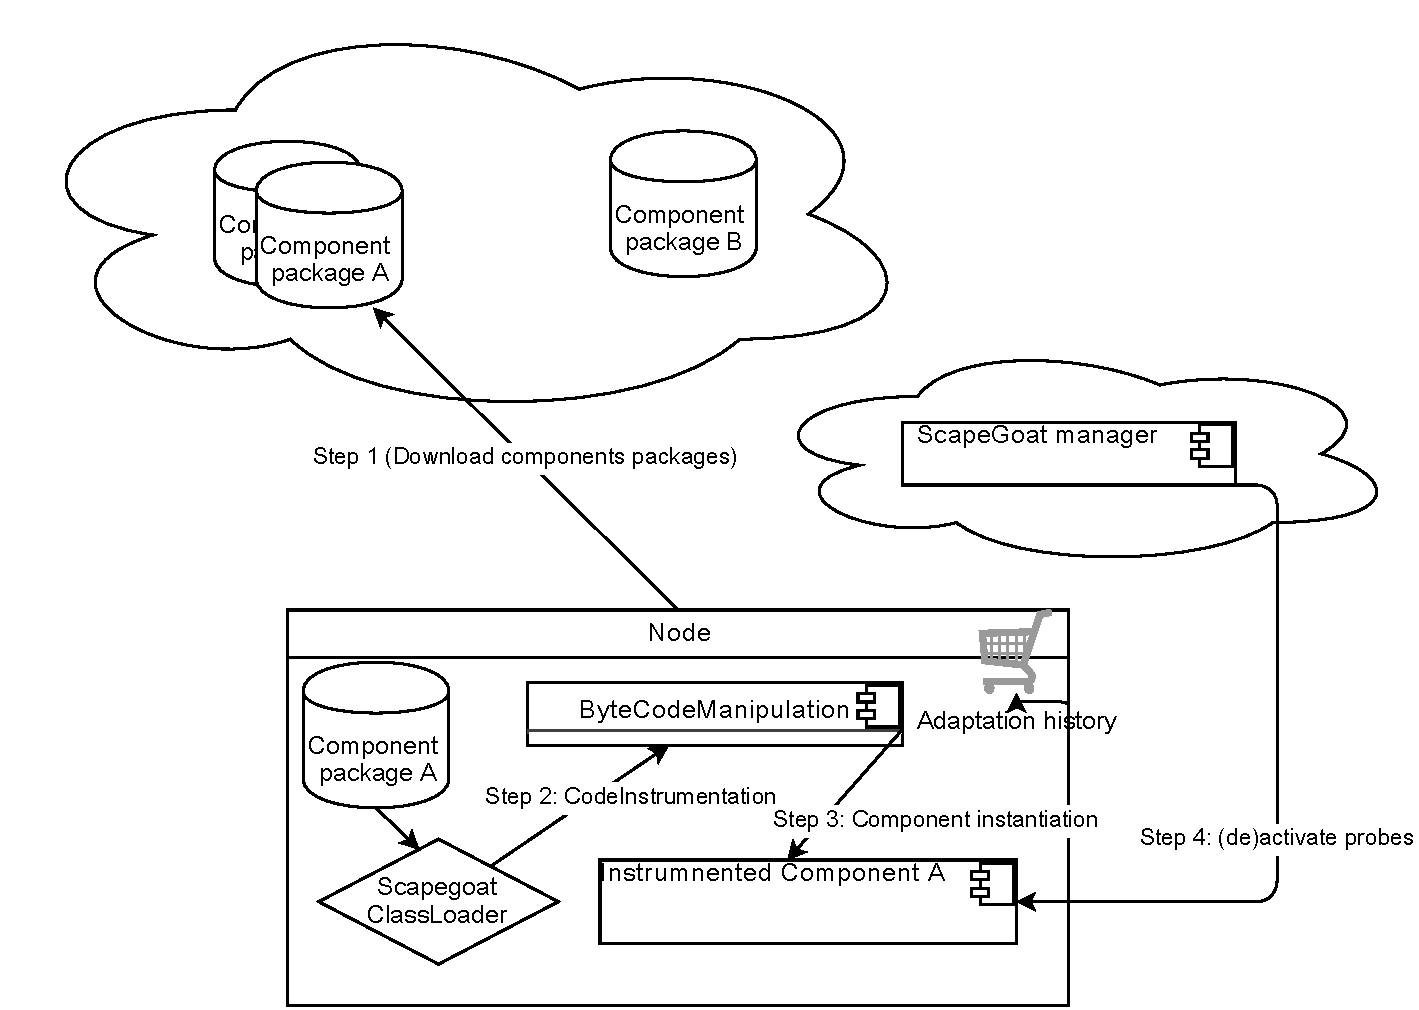
\includegraphics[scale=0.4]{figures/approach}
%	\caption{\label{fig:approach}Approach overview}
%	\end{figure}


\subsubsection{Scapegoat's architecture}

The Scapegoat framework is built using the Kevoree component framework.
Scapegoat extends Kevoree by providing a new Node Type and three new Component Types:
\begin{itemize}
\leftskip -.2in
\item \textbf{Monitored Node.}
Handles the admission of new components by storing information about resource availability.
Before admission, it checks the security policies and registers components with a contract in the monitoring framework.
Moreover, it intercepts and wraps class loading mechanisms to record a component type's loaded classes.
Such information is used later to (de)activate the probes.
\item \textbf{Monitoring Component.}
This component type is in charge of checking component contracts. 
Basically, it implements a complex variant of the algorithm in Listing \ref{algo:monitoring}.
It communicates with other components to identify suspected components.
% and to adapt the system after a fault is identified.
%todo: WHAT DOES THIS MEAN? Additionally, it makes use of another software artifact to deal with the (de)activation of probes. 
\item \textbf{Ranking Component.}
This is an abstract Component Type; therefore it is user customizable.
It is in charge of implementing the heuristic that ranks the components from the most likely to be faulty to the least likely.
\item \textbf{Adaptation component.}
This component type is in charge of dealing with the adaptation of the application when a contract violation is detected.
It is also a customizable component.
The adaptation strategy whenever a faulty component is discovered is out os scope of this thesis.
Nevertheless, several strategies may be implemented in Scapegoat, such as removing faulty components or slowing down communication between components when the failure is due to a violation in the way one component is using another.
\end{itemize}

\subsubsection{Extensibility of the Scapegoat Framework}
%\todo{For Walter: Review this section}
%\todo{We need to talk about three things: the heuristics, the admission control and the contracts semantics or implementation extensibility}

The Scapegoat framework has been built with the idea of being as generic as possible, thus supporting various extensions and specializations.
In this section we discuss the extension points provided by the Scapegoat framework.

%Defining heuristics to rank components is a part of the framework that can be specialized 
Heuristics used to rank suspected faulty components can be highly specialized
and, as we show in section~\ref{sec:evaluation}, have a remarkable impact on the behavior of Scapegoat.
A new heuristic is created by defining a component that implements an interface to provide a ranking of the suspected components.
To do so, a context is sent with each ranking request on this component.
This context is composed of three elements, 
i) a model that describes the components and links of the deployed application, 
%ii) a models' history which contains all the models that have been deployed on the platform, and 
ii) a history that contains all the models that have been deployed on the platform, and 
iii) a history of failures composed of metadata regarding what components have failed as well as why and when it happened.
In this thesis, we present three heuristics.
The first heuristic is proposed in section~\ref{sec:heuristic-based-on-modeling} and shows how we can leverage the Models@Run.time paradigm to guide the framework in finding the component that is behaving abnormally.
Due to their simplicity, the other two heuristics are presented in section~\ref{sec:evaluation} where we use them to evaluate the behavior of Scapegoat.

The mechanism for creating new heuristics is based on the strategy design pattern. Figures \ref{fig:strategy-class} and \ref{fig:strategy-sequence} illustrates this extension point. 


\begin{figure}[h!]
\centering
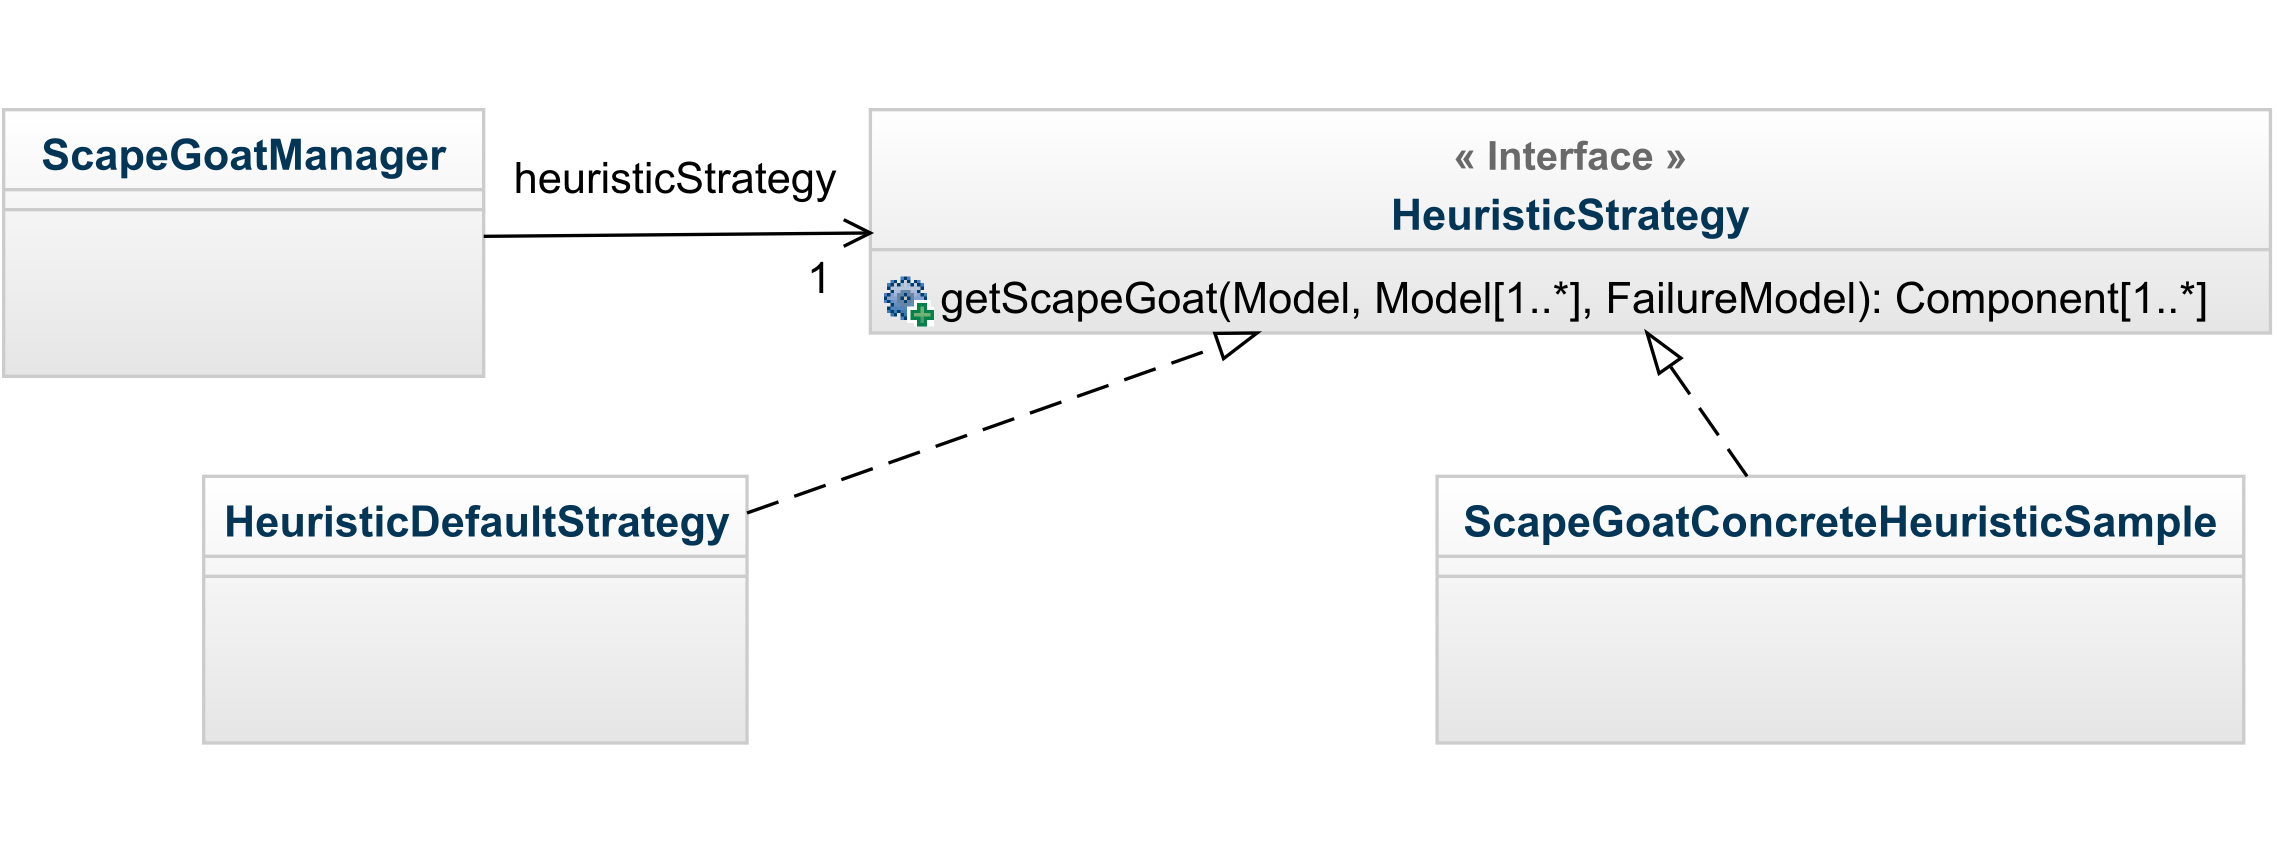
\includegraphics[width=0.9\textwidth]{./chapter5/figures/strategy-class}
\caption{\label{fig:strategy-class}Heuristic extension point in Scapegoat. This illustrates the class diagram.}
\end{figure}

\begin{figure}[h!]
\centering
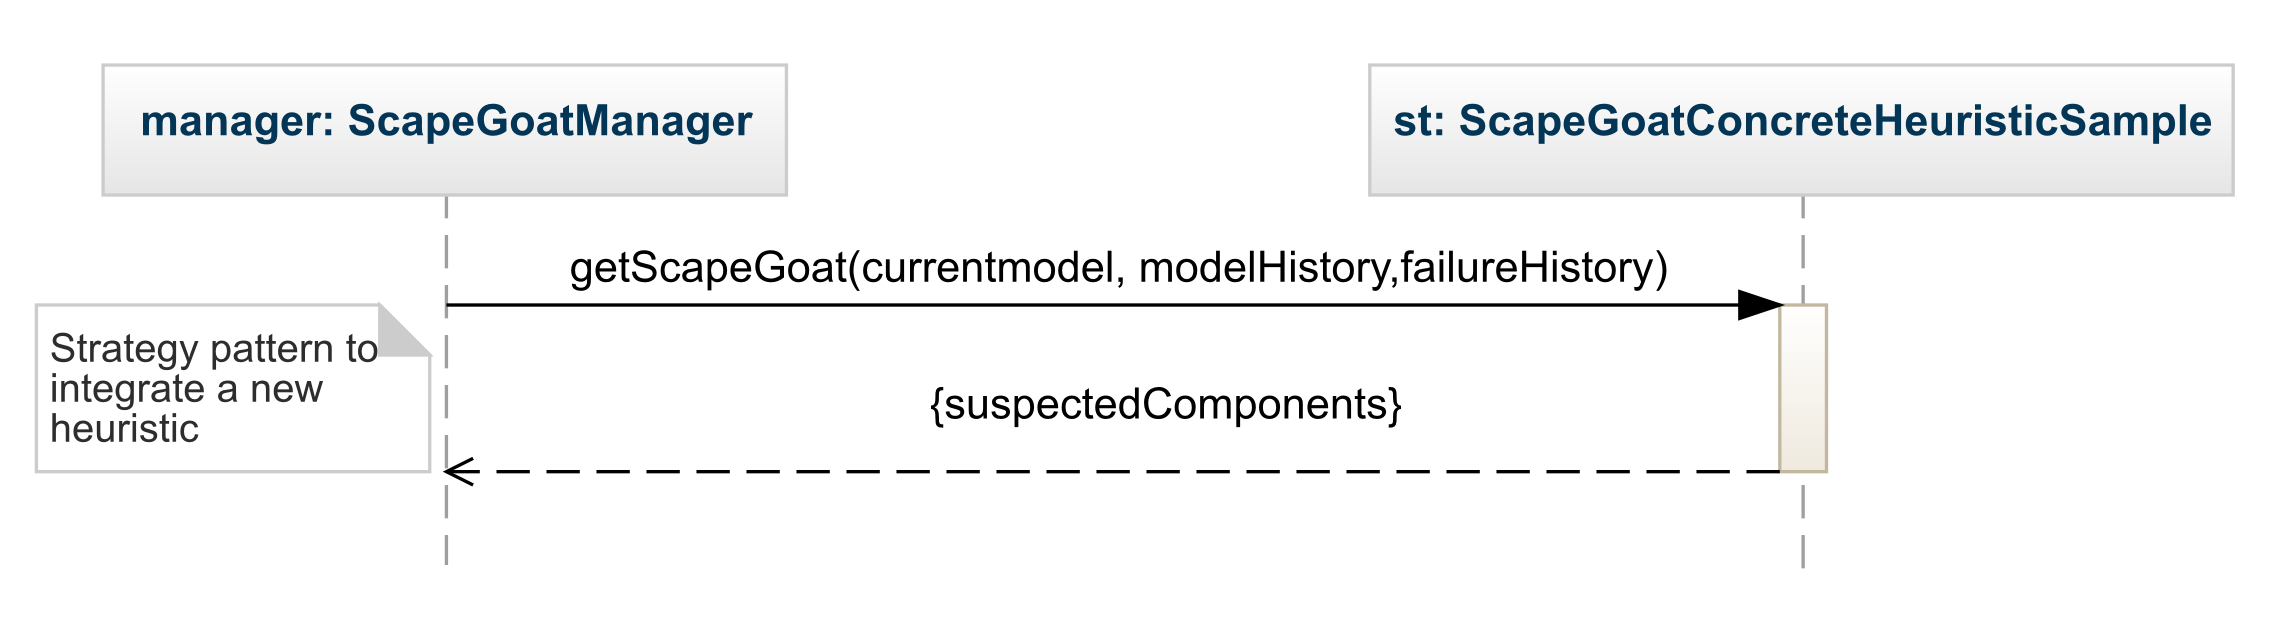
\includegraphics[width=0.9\textwidth]{./chapter5/figures/strategy-sequence}
\caption{\label{fig:strategy-sequence}A sequence diagram showing how the extension point to define heuristics in Scapegoat is used.}
\end{figure}

A second extensible aspect of the framework is the admission control system.
The framework provides an API to hook user-defined actions when new components are submitted for deployment.
Basic data describing the execution platform in terms of resource availability, information about the already deployed components and the new component's contract are sent to the user-defined admission control system.
On each request, the admission control system has to accept or refuse the new component.
We are using an approach that checks the theoretical availability of resources whenever a component is deployed, and accepts the new component if the contract can fit in the remaining available resources.
Scapegoat is meant to support other policies as, for instance, overcommitment.
 
A last element that can be specialized to user needs is the contracts semantic.
In section~\ref{componentcontract} we describe how we interpret the contract in this work.
However, it is possible to define other contract semantics, for instance, accepting values that are closed to the limit defined in the contract, or using fuzzy values instead of sharp values.
It is worth noting that modifying the semantic of the contract would likely involved redefining the domain-specific language to describe contract and also modifying the admission control system.
 
%There are many customizable features in the framework.
%Other aspects to modify are the admission control algorithm used and the logic to check if a component behaves according its contract.
%Users of the framework can also redefine the mechanism to monitor communication among components, as we do in section~\ref{sec:WebStudy}, in order to fully capture communication based on other channels.
%Finally, in a solution that really support reconfiguration, it is essential to provide adaptation strategies.


\subsubsection{Implementation strategy}
Scapegoat aims at minimizing monitoring overhead when the framework is monitoring the global behavior of the JVM. 
To achieve this, Scapegoat uses as few probes as possible when executing in global monitoring mode.
Only when it is necessary, the framework activates the required probes.
This features are implemented in the framework in three modules that are in charge of different concerns: a module to activate/deactivate the probes, a module to collect the resource usage, and a module to compute what components should be carefully monitored.
In this section we focus on the modules for activating/deactivating probes and for collecting information of resource usage because they required considerable engineering effort.
Notice, however, that this module is executed on demand when the framework already decides the monitoring mode to use and what components to monitor.

\paragraph{Module to activate/deactivate probes}
In Scapegoat  we use bytecode instrumentation to perform localized monitoring.
However, instead of doing as previous approaches that manipulate the bytecode that defines components just when the component's code is executed for the first time, we modify the bytecode many times during components' life.
Every time the monitoring mode is changed we either activate or deactivate the probes by simply inserting them in the bytecode or by removing them. 
Implementing this mechanism at per-component basis requires knowing all the classes that have been loaded for a component.
This information is kept using a dictionary in which we treat a component's id as a key and a set of class names as a value.
The dictionary is filled using the \textit{traditional} classloader mechanism of Java.
In short, when a class is loaded on behalf of a component, we detect the class name and the thread that is loading the class.
Using the thread's id we are able to identify the component because we use special naming conventions for each thread executing the initial code of a component.
When probes are activated/deactivated on a component, iterating over the set of class names allows the re-instrumentation of each involved class.

The probes perform two actions: collecting data about the local usage of resources (e.g., objects recently allocated, instructions executed in the current basic block, bytes sent through the network), and notifying to the resource consumption monitor about the collected data. 
Some data we collect is computed statically when the bytecode is loaded.
This includes the size of each basic block and the size of each object allocated when the size of each instance of the class is already known.
Other data, such as bytes sent through the network or the size of allocated arrays, can only by collected dynamically when the code is running.
To notify about the collected data we use simple method calls to a proxy class in charge of forwarding the data to the monitoring module.
Probes to detect CPU consumption are inserted at the end of each basic block.
These probes collect the size in number of instructions of its container basic block.
Probes for IO throughput and network bandwidth are added in a few selected method defined in classes of the Java Development Kit (JDK).
These probes take the needed information from local variables (e.g., number of bytes) and call the proxy class. 

Our implementation, which is built using the ASM library~\footnote{asm.ow2.org} for bytecode manipulation and a Java agent to get access to and transform the classes, is based on previous approaches to deal with resource accounting and profiling in Java~\cite{binder_portable_2006,Binder200645,czajkowski_jres:_1998}.
As in previous approaches, we compute the length of each basic block to count the number of executed instructions and we try to keep a cache of \textit{known} methods with a single basic block.
Moreover, we compute the size of each object once it is allocated and we use \textit{weak} references instead of \textit{finalizers} to deal with deallocation.

\paragraph{Module to collect information regarding resource usage}
In Scapegoat, there are two mechanisms to collect information about how components consume resources.

The first mechanism is able to capture the usage of CPU, IO throughput, network bandwidth and memory.
Every time a probe that was inserted in the code of a component is executed, the proxy class forwards the local resource usage to the module in charge of collecting the resource usage.
Along with the local resource usage, probes also notify the id of the components consuming resource.
Such data is then used to aggregate the global consumption of each component.
It is worth noting that, when this first mechanism is used to collect memory consumption, on object is always accounted as  consumed for the component responsible for its initial allocation.
In short, no matter whether the initial component $C$ that allocates the object no longer held a reference to an object $O$, as long as $O$ remains in memory, $C$ is accounted for its consumption.
Moreover, as was already mentioned, using this mechanism is not possible to deactivate the probes related to memory consumption.

On the contrary, the second mechanism is only useful to collect information about memory consumption.
The advantages of this method are: we can leverage the proposed optimistic monitoring because it executes only on demand, and it has no impact on the number of objects allocated in memory because no \textit{weak references} are used.
However, in this method an object $O$ is consumed not for the component that allocates it but for those components that held references to it.
As a consequence, in certain occasions the framework states that an object is being consumed for many components at the same time. 
We built this solution on top of JVMTI by implementing the algorithm proposed in~\cite{Price:2003:GCM:829515.830545, dsn/09/geoffray/ijvm}, with the main difference being that our solution works without modifying the garbage collector.
In summary, this algorithm simply try to find those objects that are reachable from the references of each component.
It does so by traversing the graph of live object using as the component instance and its threads as roots of the traversal. 
Since our approach does not require a modification to the garbage collector, it is portable and works with different garbage collector implementations.

%\subsubsection{Quality of Contract} 

%\todo{}
%\todo{do not forget to have a part on implementation}

\subsection{Leveraging Models@run.time to build an efficient monitoring framework}\label{sec:heuristic-based-on-modeling}
As presented in section \ref{monitorContainer}, our approach offers a dynamic way to activate and deactivate fine-grain localized monitoring.
We use a heuristic to determine which components are more likely to be faulty.
Suspected components are the first to be monitored.

%\hl{Isn't this a conclusion of the evaluation? Why is it here?}
%When compared to fine-grain monitoring of all components, our technique decreases the accumulated overhead of the monitoring system when a problem is detected.
%It should be noted that a poorly performing heuristic may introduce extensive delays in identifying faulty components.
%With this in mind, our approach is a trade-off between low monitoring overhead and the delay introduced to identify the faulty component (i.e., overhead versus latency).
%Thus, the overall performance of our approach is tightly coupled to the performance of our heuristic in accurately finding faulty components.

Our framework supports the definition of different heuristics, which can be application or domain-specific.
In this chapter we propose a heuristic that leverages the use of the Models@run.time approach to infer the faulty components.
The heuristic is based on the assumption that the cause of newly detected misbehavior in an application is likely to come from the most recent changes in the application.
This can be better understood as follows:
\begin{itemize}
\leftskip -.2in
  \item recently added or updated components are more likely to be the source of a faulty behaviour;
  \item components that directly interact with recently added or updated components are also suspected.
\end{itemize}

We argue that when a problem is detected it is probable that recent changes have led to this problem, or else, it would have likely occurred earlier.
If recently changed components are monitored and determined to be healthy, it is probable that the problem comes from direct interactions with those components.
Indeed, changes to interactions can reveal dormant issues with the components.
The algorithm used for ranking the components is presented in more detail in Listing \ref{algo:heuristic}.
%todo: WHAT???? Note that in this heuristic, each subset of components to be finely monitored is composed for one element of the list.
In practice, we leverage the architectural-based history of evolutions of the application, which is provided by the Models@run.time approach.
%The heuristic starts at the most recently changed components, because they are more likely to have introduced the problem, and we iteratively move to older components.


\begin{lstlisting}[escapeinside={(*}{*)},caption=The ranking algorithm (uses the model history for ranking).,label=algo:heuristic,float=!h]
ranker() : list<Component>
	// used to avoid adding duplicated elements to the list
	visited = (*$\emptyset$*)
	// this list will contain the result of calling the routine
	ranking = {}
	for each model M (*$\in$*) History
		// adding components that were added in this model
		N = {c (*$\mid$*) c was added in M}
		ranking.add N(*$\setminus$*)visited
		visited = visited (*$\cup$*) N
		// finding neighbors
		Neighbors (*$ = \bigcup_{c \in N}{c.neighbors}$*)
		SortedNeighbors = sort (Neighbors (*$\setminus$*) visited, History)
		// adding neighbors
		ranking.add SortedNeighbors
		visited = visited (*$\cup$*) Neighbors
	// return the built ranking
	return ranking

// this routine recursively sort a set of components using the following criteria:
// components are sorted by the timestamp that indicates when they were installed
private sort (S : Set<Component>, H : History) : list<Component>
	r = {}
	if (*$S \ne \emptyset$*)
		choose (*$b \mid b \in S$*) (*$\wedge$*) b is newer with respect to H than any other element in S
		r.add b, sort (S(*$\setminus$*){b}, H)
	return r
\end{lstlisting}

Listing~\ref{algo:heuristic} shows two routines, but only routine \textit{ranker} is public.
It can be called by the monitoring system when it is necessary to figure out in what order components must be carefully monitored. 
After initializing an empty list which will hold the rank, the algorithm starts to iterate in line 6 over the history of models that have been installed in the system.
As mentioned, this history contains a sorted set of models that describe what components have been installed in the system.
Within each iteration, the algorithm first computes in line 8 the set of components that were installed at such a point in time.
Afterwards, these components are added to the result.
The next step, executed at lines 12 and 13, is finding those components that are directly connected to components that were added to the application at this point in time.
Finally, these \textit{neighbors} are added to the rank after being sorted.
Routine \textit{sort} simply sorts a set of components using as criteria the time at which components where installed in the system.

%We implemented this alogrithm using the kevoree framework that provide the model to know the interactions between components and which offer access to the model history.
%\subsection{Analysis of expected behaviour}\label{analysis}
%
During adaptive monitoring, the monitoring system transits between either \textit{Global} lightweight monitoring (G) and \textit{All Components} or full monitoring (F), or Global and \textit{Specific} monitoring based on heuristics (H).
We can describe the transitions back and forth as:
\begin{subequations}
\begin{align}
G \rightarrow F \label{tA1}
\\F \rightarrow G \label{tA2}
\end{align}
\end{subequations}
\begin{subequations}
\begin{align}
G \rightarrow H \label{tH1}
\\ H \rightarrow G \label{tH2}
\end{align}
\end{subequations}
Different monitoring modes have different times to detect a failure.
We denote by $T_{df}(F),T_{df}(G),T_{df}(M_x)$ the time to detect failure of full, global and subset monitoring respectively. 
We know by construction that relations \eqref{dt0}, \eqref{dt1} and \eqref{dt2} hold.
This means that full monitoring should detect both the existence of a fault and the source of a fault faster than adaptive monitoring because all components are continuously checked instead of just a lightweight global check\footnote{It should be noted that the lightweight global monitoring mode can only detect the existence of a fault but not the source of the fault. To detect the source of the fault, more intrusive, per-component monitoring is required}.
However, there is no direct relationship between the two variants of adaptive monitoring (i.e., \eqref{dt1} and \eqref{dt2}) because the delay depends on the time needed to probe and instrument components (varies according to the number and size of classes), and the quality of the heuristic in targeting faulty components as quickly as possible.
The former element affects the delay when \textit{all components} are instrumented.
The latter depends on the ability of the heuristic to include the faulty component inside the set of suspected faulty components.
\begin{subequations}
\begin{align}
T_{df}(F) \le T_{df}(G) \label{dt0}
\\ T_{df}(F) \le T_{df}(G) + \sum_{i=0}^{j}(T_{trans}(C_i) + T_{df}(M_i)) \label{dt1}
\\ T_{df}(F) \le T_{df}(G) + T_{trans}(all) + T_{df}(M_{all}) \label{dt2}
\end{align}
\end{subequations}
%The experiments have shown the impact of monitoring policies over performance.
Another important dimension is the global overhead of each policy on the running system.
The following relations apply to this dimension.
Relation \eqref{overheadRelations1} is true because Full monitoring is always costlier than lightweight Global monitoring.
Relations \eqref{overheadRelations2} and \eqref{overheadRelations3} are true if a single faulty behaviour occurs during the execution of the application.
However, these relations do not apply when the number of failures and the number of transitions grow.
It is also impossible to establish a relation between the two adaptive monitoring policies because, once again, it depends on the size of the application and the quality of the heuristic in quickly finding the source of faults. 
\begin{subequations}
\begin{align} 
 O(F) > O(G) \label{overheadRelations1}
\\ O(F) > O(G) + O_{trans}(all) + O(M_{all}) \label{overheadRelations2}
\\ O(F) > O(G) + \sum_{i=0}^{j}(O_{trans}(C_i) + O(M_i)) \label{overheadRelations3}
\end{align}
\end{subequations}
Only relationship \eqref{overheadRelations1} is independent of the application.
The other relationships depend on time.
We can express overhead as a time dependent function.
For instance, let $O_F(t)$,  $O_A(t)$ be the overhead in the application due to Full monitoring and Adaptive monitoring with all components respectively.
Where: 
\begin{equation*}
O_F(t)\approx const
\end{equation*}
\begin{equation*} 
O_A(t) = 
	\begin{cases}
   		O(G) & \text{if in G state} \\
   		O_{trans}(all) & \text{if changing state in t} \\
   		O(M_{all})=O(F) & \text{if in A state}
  	\end{cases} 
\end{equation*}
The integral expresses the overhead in a given amount of time.
The relation \eqref{eq:overhead-time} is true under two conditions.
On the one hand, if time spent in global monitoring is bigger than time spent in other states.
On the other hand, if the overhead due to transitions is small.
A similar analysis is applicable to adaptive monitoring based on heuristics.
\begin{equation}
\int O_F(t)\,dt > \int O_A(t)\,dt \label{eq:overhead-time}
\end{equation}
The first condition is reasonably met through the two following factors.
First, we can expect that most applications have few failures in comparison to the global execution time of the application.
Second, the application container should provide an adaptation mechanism to remove the source of failure when a contract violation is identified.
This adaptation would allow the system to transition back into global monitoring.

Following the previous analysis we can conclude that the overhead of the monitoring framework depends on the following factors: the time spent in global monitoring, the number of transitions performed to intrusive monitoring, the quality of the heuristic, and the size of the application.
Likewise, the quality of the heuristic and the size of the application affect the delay to detect failures.
%We can now see that the behavior of \textit{all monitoring} strategy is due to the hostile execution environment we are using.
%The behavior change completely if we introduce an adaptation mechanism to remove the faulty component instead of allowing the its uncontrolled execution.



\section{ScapeGoat Performance Evaluation\label{sec:evaluation}}
In this section we present a first series of experiments and discuss the usability of our approach.
We focus on the following research questions to assess the quality and the efficiency of ScapeGoat:

\begin{itemize}
	\item \textbf{What is the impact of the various levels of instrumentation on the application?}
	Our approach assumes high overhead for full monitoring and low overhead for a lightweight global monitoring system. The experiments presented in section \ref{sec:OverheadFullMonitoring} show the overhead for each instrumentation level.
	\item \textbf{What is the performance cost of using instrumentation-based and heap-exploration-based memory monitoring?}
	Since both mechanisms have by design different features, the experiments in section \ref{sec:OverheadFullMonitoring} show the overhead each mechanism produces. 
	\item \textbf{Does our adaptive monitoring approach have better performance than state-of-the-art monitoring solutions?}
	The experiment presented in section \ref{sec:adaptive-vs-full} highlights the performances benefits of our approach considering a real-world scenario.
	\item \textbf{What is the impact of using a heuristic in our adaptive monitoring approach?}
	The experiment presented in section \ref{sec:switch-heuristic} highlights the impact of the application and component sizes, and the need of a good heuristic to quickly identify faulty components.
%Our last experiments aims at showing the potential benefits of the Heuristics in our approach. The experiment presented in section \ref{heuristic_eval} highlights the benefits of using a heuristics with a growing size of the application.
\end{itemize}

The efficiency of our monitoring solution is evaluated on two dimensions: the overhead on the system and the delay to detect failures.
We show there is a trade-off between the two dimensions and that ScapeGoat provides a valuable solution that increases the delay to detect a faulty component but reduces accumulated overhead.
This evaluation has been conducted on a Cyber Physical System case study.
It corresponds to a concrete application that leverage the Kevoree framework for dyamic adaptation purpose.

We have built several use cases based on a template application from our motivating example in section \ref{sec:scapegoat-motivaing-example}.
We reused an open-source crisis-management application for firefighters that has been built with Kevoree components.
We use two functionalities of the crisis-management application.
The first one is for managing firefighters.
The equipment given to each firefighter contains a set of sensors that provides data for the firefighter's current location, his heartbeat, his body temperature, his acceleration movements, the environmental temperature, and the concentration of toxic gases. 
These data are collected and displayed in the crisis-management application, which provides a global-view of the situation. 
The second functionality uses drones to capture real-time video from an advantageous point-of-view.

Figure \ref{fig:complete-usecase} shows the set of components that are involved in our use-case, including components for firefighters, drones and the crisis-management application\footnote{More information about these components is given in \url{http://goo.gl/x64wHG}}. The components in the crisis-management application are used in our experiments, but the physical devices (drones and sensors) are simulated through the use of mock components.
The application presents two components: the first one is a web browser that shows information about each firefighter in the terrain, and the second one allows to watch the video being recorded by any drone in the field.
A Redis database is used to store the data that is consumed for the application's GUI.

\begin{figure*}[!bt]
	\centering
	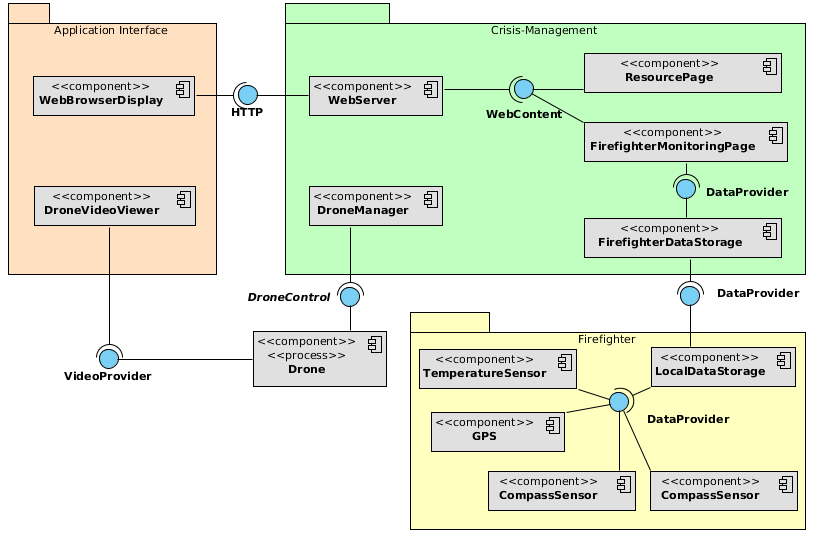
\includegraphics[scale=0.4]{./chapter5/figures/complete-usecase-new2}
	\caption{\label{fig:complete-usecase}The component configuration for our crisis-management use-case.}
\end{figure*}

Every use case we present extends the crisis-management base application by any one of the following possibilities: adding new or redundant components, adding external Java applications with wrapper components (e.g., Weka, DaCapo), or modifying existing components (e.g., to introduce a fault into them).
Using this template in the experiments allow us to measure the behavior of our proposal in a more realistic environment where many components with different features co-exist.
%is extended in every use case by: modifying existent components (e.g, to introduce faulty behavior), adding new redundant components and adding external java applications with a wrapper component.
%The particular features of each component are details in each experiment.

\subsection{Measurement Methodology} \label{sec:measurement_metodology}
To obtain comparable and reproducible results, we used the same hardware across all experiments: a laptop with a 2.90GHz Intel(R) i7-3520M processor, running Fedora 19 with a 64 bit kernel and 8GiB of system memory.
We used the HotSpot Java Virtual Machine version 1.7.0\_67, and Kevoree framework version 5.0.1.
Each measurement presented in the experiment is the average of ten different runs under the same conditions. 
%In addition to the template application we presented, we introduce a new component to execute an external jar file. This new component is used to measure the impact of the faulty behavior on the execution of the system by measuring its execution time.

The evaluation of our approach is tightly coupled with the quality of the resource consumption contracts attached to each component.
We built the contracts following classic profiling techniques. 
The contracts were built by performing several runs of our use cases, without inserting any faulty components into the execution.
Firstly, we executed the use cases in an environment with global monitoring activated to get information for the global contract.
Secondly, per-component contracts were created by running the use cases in an environment with full monitoring.

\subsection{Overhead of the instrumentation solution\label{sec:OverheadFullMonitoring}}
Our first experiment compares the various instrumentation levels to show the overhead of each one. 
In this section, \emph{Memory instrumentation} refers to the technique for accounting memory which leverage bytecode instrumentation, while \textit{Heap Exploration} refers to the memory accouting technique which leverage on-demand heap exploration.
%The results of the evaluation are fundamental because they justify the interest of our adaptative monitoring approach. 
%Additionally, these results are the baseline to understand the rest of the evaluation. 
In this experiment, we compare the following instrumentation levels: \emph{No monitoring}, \emph{Global monitoring}, \emph{Memory instrumentation}, \emph{Instructions instrumentation}, \emph{Memory and instructions instrumentation} (i.e., Full monitoring).
We also evaluate the impact on performance of the two fine-grain memory monitoring approaches we proposed: instrumentation-based and heap-dump-based.

In this set of experiments we used the DaCapo 2006 benchmark suite \cite{Blackburn:2006:DBJ:1167473.1167488}. 
We developed a Kevoree component to execute this benchmark~\footnote{\url{http://goo.gl/V5T6De}}.
The container was configured to use full monitoring and the parameters in the contract are upper bounds of the real consumption\footnote{Scripts are generated from those available at \url{http://goo.gl/FR8LC7}.}.

\begin{figure}[!ht]
\centering
\begin{tikzpicture}
\begin{axis}[
every axis legend/.append style={nodes={right}},
ybar=0pt,
legend style={at={(0.25,1.1)},
anchor=north,legend columns=1, font=\tiny},
ylabel={Time (seconds)},
y label style={at={(0.04, 0.5)}},
scaled y ticks = false,
      y tick label style={/pgf/number format/fixed,
      /pgf/number format/1000 sep = \thinspace % Optional if you want to replace comma as the 1000 separator 
      },
xtick=data,ymin=0,
width = 13cm,
height = 5cm,
bar width = 6,
x tick label style={rotate=45,anchor=east, font=\small},
 axis lines*=left, % Don't display the top and right lines
 symbolic x coords={antlr,fop,hsqldb,jython,chart,luindex,xalan,lusearch}
]
\addplot[fill=black] coordinates 
	{(antlr,1.28) (fop,1.101) (hsqldb,2.337) (jython,2.351) (chart,2.534) (luindex,3.561) (xalan,1.224) (lusearch,1.305)};
\addplot[fill=gray] coordinates 
	{(antlr,1.023) (fop,1.039) (hsqldb,2.284) (jython,2.524) (chart,2.417) (luindex,3.165) (xalan,1.191) (lusearch,1.321)};
\addplot[pattern=north east lines] coordinates 
	{(antlr,2.164) (fop,1.188) (hsqldb,8.655) (jython,10.688) (chart,4.806) (luindex,8.001) (xalan,4.885) (lusearch,9.349)};
\addplot[pattern=crosshatch] coordinates 
	{(antlr,6.235) (fop,1.905) (hsqldb,9.091) (jython,10.905) (chart,8.985) (luindex,44.988) (xalan,8.026) (lusearch,9.261)};
\addplot[pattern=dots] coordinates 
	{(antlr,7.468) (fop,1.970) (hsqldb,15.888) (jython,18.625) (chart,11.502) (luindex,51.660) (xalan,11.188) (lusearch,18.975)};
\legend{No monitoring, Global monitoring, Memory instrumentation,Instructions instrumentation, Memory \& Instructions instrumentation}
\end{axis}
\end{tikzpicture}
\caption{Execution time for tests using the DaCapo Benchmark\label{overhead-of-monitoring}}
\end{figure}

Figure \ref{overhead-of-monitoring} shows the execution time of several DaCapo tests under different scenarios when only instrumentation is used to provide fine-grain monitoring.
First, we wish to highlight that \emph{Global monitoring} introduces no overhead compared with the \emph{No monitoring} mode.
Second, the overhead due to memory accounting is lower than the overhead due to instruction accounting.
This is very important because, as we described in section \ref{monitorContainer}, memory probes cannot be deactivated dynamically.

To perform the comparison, we evaluate the overhead produced for each monitoring mode. We calculated the overhead as: \[overhead=\frac{WithInstrumentation}{GlobalMonitoring}\]

The average overhead due to instruction accounting is 5.62, while the value for memory accounting depends on the monitoring mechanism.
If bytecode instrumentation is used, the average overhead is 3.29 which is close to the values reported in \cite{Binder:2009:PPV:1464245.1464249}.
In the case of instruction accounting, these values are not as good as the values reported in \cite{Binder:2009:PPV:1464245.1464249}; because they obtain a better value between 3.2 and 4.3 for instructions accounting.
The performance difference comes from a specific optimization that we chose not to apply.
The optimization provides fast access to the execution context by adding a new parameter to each method.
Nevertheless, this solution needs to keep a version of the method without the new parameter because native calls cannot be instrumented like that. 
We decided to avoid such an optimization because duplication of methods increases the size of the applications, and with it, the memory used by the heap.
In short, our solution can reach similar values if we include the mentioned optimization, but at the cost of using more memory.
On the other hand, the values we report are far lower than the values reported in \cite{Binder:2009:PPV:1464245.1464249} for hprof.
Hence, we consider that our solution is comparable to state of the art approaches in the literature.

In Figure~\ref{overhead-of-monitoring-with_heapexplorer} we compare the execution time of the same benchmarks but using different memory monitoring approaches.
This comparison is important because, as explained in section~\ref{monitorContainer}, the two approaches have different CPU footprint.
These are controlled experiments where, in order to stress the technique, we demand the execution of a \textit{heap exploration} step every two seconds, which is not the expected usage pattern.
On the contrary, the memory instrumentation technique is executed with the expected usage pattern.
In comparison to using memory instrumentation where the average execution time is 3.29, the average overhead in execution time  decreases to 1.79 if the \textit{Heap Exploration} monitoring mechanism is used.
This value is better than the value reported in \cite{Binder:2009:PPV:1464245.1464249}.
These results suggest that this technique has less impact on the behavior of applications being monitored.

\begin{figure}[!ht]
\centering
\begin{tikzpicture}
\begin{axis}[
every axis legend/.append style={nodes={right}},
ybar=0pt, legend style={at={(0.25,1.1)},
anchor=north,legend columns=1, font=\tiny},
ylabel={Time (seconds)},
y label style={at={(0.04, 0.5)}},
scaled y ticks = false,
      y tick label style={/pgf/number format/fixed,
      /pgf/number format/1000 sep = \thinspace % Optional if you want to replace comma as the 1000 separator 
      },
xtick=data,ymin=0,
width = \textwidth,
height = 5cm,
bar width = 6,
x tick label style={rotate=45,anchor=east, font=\small},
 axis lines*=left, % Don't display the top and right lines
 symbolic x coords={antlr,fop,hsqldb,jython,chart,luindex,xalan,lusearch}
]
% no monitoring
\addplot[fill=black] coordinates 
	{(antlr,1.28) (fop,1.101) (hsqldb,2.337) (jython,2.351) (chart,2.534) (luindex,3.561) (xalan,1.224) (lusearch,1.305)};
% memory
\addplot[pattern=north east lines] coordinates 
	{(antlr,2.164) (fop,1.188) (hsqldb,8.655) (jython,10.688) (chart,4.806) (luindex,8.001) (xalan,4.885) (lusearch,9.349)};
% heap dump
\addplot[pattern=crosshatch dots] coordinates 
	{(antlr,1.143) (fop,1.125) (hsqldb,8.639) (jython,2.762) (chart,2.836) (luindex,3.589) (xalan,1.822) (lusearch,5.078)};
% memory and instructions
\addplot[pattern=dots] coordinates 
	{(antlr,7.468) (fop,1.970) (hsqldb,15.888) (jython,18.625) (chart,11.502) (luindex,51.660) (xalan,11.188) (lusearch,18.975)};
% heap dump and instructions
\addplot[fill=white] coordinates 
	{(antlr,6.159) (fop,1.188) (hsqldb,14.647) (jython,10.950) (chart,9.059) (luindex,44.758) (xalan,7.812) (lusearch,15.990)};
% legend
\legend{No Monitoring, Memory instrumentation, Heap Exploration, Memory \& Instructions instrumentation, Heap Exploration \& Instructions Instrumentation}
\end{axis}
\end{tikzpicture}
\caption{Comparison of execution time for tests using two different memory monitoring techniques\label{overhead-of-monitoring-with_heapexplorer}}
\end{figure}

The results of our experiment shown in Figures~\ref{overhead-of-monitoring} and~\ref{overhead-of-monitoring-with_heapexplorer} demonstrate the extensive impact of the \emph{Full monitoring} mode, which uses either \emph{Memory instrumentation} or \emph{CPU instrumentation}, has on the application. Thus, our \emph{Adaptive monitoring} mode, which uses \emph{Global monitoring} and switches to \emph{Full monitoring} or \emph{localized monitoring}, has the potential to reduce this accumulated overhead due to the fact that \emph{Global monitoring} has no appreciable overhead. 
%The results of the evaluation are fundamentals because they justify the interest of our adaptative monitoring approach. 
%Additionally, these results are the baseline to understand the rest of the evaluation. 

%In addition, we plan to study alternatives to improve instruction accounting. %These alternatives are about using peak monitoring and learning monitoring.
%For example, we plan to study the use of machine learning for monitoring \cite{tesauro2006hybrid}. Based on a machine learning approach, it is possible to train the monitoring system to do the instruction instrumentation. Then, instead of doing normal instruction instrumentation, we might only do, for example, method-calls instrumentation and with the learning data, the monitoring system should be able to infer the CPU usage of each call, whilst lowering the overhead.

\subsection{Overhead of Adaptive Monitoring vs Full Monitoring\label{sec:adaptive-vs-full}}
The previous experiment highlights the potential of using \emph{Adaptive monitoring}. However, switching from \emph{Global monitoring} to either \emph{Full} or \emph{Localized monitoring} introduces an additional overhead due to having to instrument components and activate monitoring probes.
Our second experiment compares the overhead introduced by the adaptive monitoring with the overhead of \emph{Full monitoring} as used in state-of-the-art monitoring approaches. 
%The result of this experiment shows the potential interest of the adaptive monitoring approach.

Table \ref{use-cases-sheet2} shows the tests we built for the experiment.
We developed the tests by extending the template application. Faults were introduced by modifying an existing component to break compliance with its resource consumption contract.
We reproduce each execution repetitively; thus, the faulty behaviour is triggered many times during the execution of the application. The application is not restarted.
%\hl{We selected as heuristic in almost every case \textit{number-of-failures} which is the best because there is only a single faulty component.}\todo{must be explain later}

\begin{table*}[!hb]
\centering
\caption{Features of use cases.\label{use-cases-sheet2}}
\begin{tabular}{|c|p{2.1cm}|p{1.4cm}|p{2cm}|p{2.5cm}|}
\hline Test Name & Monitored\newline Resource & Faulty\newline Resource & Heuristic & External Task \\ 
\hline UC1 & CPU, Memory & CPU & number\newline of failures & Weka, training neural network \\ 
\hline UC2 & CPU, Memory & CPU & number\newline of failures & dacapo, antlr \\ 
\hline UC3 & CPU, Memory & CPU & number\newline of failures & dacapo, chart \\ 
\hline UC4 & CPU & CPU & number\newline of failures & dacapo, xalan \\ 
\hline UC5 & CPU, Memory & CPU & less number\newline of failures\newline first  & dacapo, chart \\ 
\hline UC6 & Memory & CPU & number\newline of failures & Weka, training neural network \\ 
\hline 
\end{tabular} 
\end{table*}


Figure \ref{adaptive-vs-full} shows the execution time of running the use cases with different scenarios.
Each scenario uses a specific monitoring policy (\emph{Full monitoring}, \emph{Adaptive monitoring with All Components}, \emph{Adaptive monitoring with Localized monitoring}, \emph{Global monitoring}).
All these scenarios were executed with the heap explorer memory monitoring policy. 
This Figure shows that the overhead differences between \textit{Full monitoring} and \emph{Adaptive monitoring with All Components} is clearly impacted by scenarios that cause the system to transition too frequently between a lightweight Global and a fine-grain \emph{Adaptive monitoring}.
Such is the case for use cases UC3 and UC4 because the faulty component is inserted and never removed.
%As we explained in section \ref{analysis}, 
Using \emph{Adaptive monitoring} is beneficial if the overhead of \emph{Global monitoring} plus the overhead of switching back and forth to \emph{All Components monitoring} is less than the overhead of the \emph{Full monitoring} for the same execution period.
If the application switches between monitoring modes too often then the benefits of adaptive monitoring are lost.

The overhead of switching from \emph{Global monitoring} to \emph{full components} or \emph{Localized monitoring} comes from the fact that the framework must reload and instrument classes to activate the monitoring probes.
Therefore, using \emph{Localized monitoring} reduces the number of classes that must be reloaded.
This is shown in the third use-case of Figure~\ref{adaptive-vs-full}, which uses a heuristic based on the number of failures.
Because we execute the faulty component many times, the heuristic is able to select, monitor and identify the faulty component quickly. This reduces overhead by 93\%. We use the following equation to calculate overhead:

\[ Gain=100-\frac{OurApproach-GlobalMonitoring}{FullMonitoring-GlobalMonitoring}*100 \]

We also evaluate the execution time for each use case using the instrumentation-based memory monitoring mode.
The average gain in that case is 81.49\% and, as shown in previous section, in average it behaves worse than the \textit{Heap Exploration} mechanism.
However, it is worth noting that the difference between using memory monitoring based on instrumentation and heap exploration is less remarkable than in the previous experiment.
Observe how in test UC4, using a combination of heap exploration and adaptive monitoring with all components behaves worse than using plain instrumentation-based memory monitoring.
In this particular test, activating and deactivating the monitoring probes dominate the execution time.
Alas, adding a heap exploration step right after the probes are activated, just add some extra overhead.
On the contrary, there is no additional step executed when we use instrumentation to measure the memory usage.
Apparently, what matter when the all components strategy is guiding the adaptive monitoring is the ratio among the amount of allocations performed by components and the size of those components.

\begin{figure}
\centering
\begin{tikzpicture}
\begin{axis}[
every axis legend/.append style={nodes={right}},
ybar=0pt, legend style={at={(0.8,1.2)},
anchor=north,legend columns=1, font=\tiny},
ylabel={Time (seconds)},
y label style={at={(0.02, 0.5)}},
scaled y ticks = false,
      y tick label style={/pgf/number format/fixed,
      /pgf/number format/1000 sep = \thinspace % Optional if you want to replace comma as the 1000 separator 
      },
xtick=data,ymin=0,
width = \textwidth,
height = 5cm,
bar width = 6,
x tick label style={rotate=45,anchor=east, font=\small},
 axis lines*=left, % Don't display the top and right lines
 symbolic x coords={UC1,UC2,UC3,UC4,UC5,UC6}
]
% full monitoring
\addplot[fill=black] coordinates 
	{(UC1,613.000) (UC2,46.363) (UC3,63.899) (UC4,78.324) (UC5,49.144) (UC6,132.949)};
% adaptive with all component
\addplot[fill=red, pattern=crosshatch dots] coordinates 
	{(UC1,432.744) (UC2,70.501) (UC3,198.554) (UC4,187.036) (UC5,32.340) (UC6,127.711)};
% adaptive with all component and heap dump
\addplot[fill=yellow, pattern=crosshatch] coordinates 
	{(UC1,410.790) (UC2,61.808) (UC3,95.503) (UC4,204.479) (UC5,16.864) (UC6,123.381)};
% adaptive with heuristic
\addplot[fill=green, pattern=north west lines] coordinates 
	{(UC1,176.413) (UC2,16.741) (UC3,29.461) (UC4,19.470) (UC5,27.001) (UC6,123.813)};
% adaptive with heuristic and heap dump
\addplot[fill=pink, pattern=dots] coordinates 
	{(UC1,169.467) (UC2,12.520) (UC3,16.403) (UC4,20.251) (UC5,15.110) (UC6,124.294)};
% global monitoring
\addplot[fill=cyan, pattern=north east lines] coordinates 
	{(UC1,166.759) (UC2,10.646) (UC3,14.37) (UC4,20.860) (UC5,14.77) (UC6,120.16)};
\legend{
	Full monitoring, 
	Adaptive with All Components using Memory Instrumentation, 
	Adaptive with All Components using Heap Exploration, 
	Localized monitoring using Memory Instrumentation, 
	Localized monitoring using Heap Exploration,
	Global Monitoring}
\end{axis}
\end{tikzpicture}
\caption{Execution time for some use cases under different monitoring policies.}\label{adaptive-vs-full}
\end{figure}

\subsection{Overhead from switching monitoring modes, and the need of a good heuristic\label{sec:switch-heuristic}}
As we explain in the previous experiments, even if using \emph{Localized monitoring} is able to reduce the overhead of the monitoring system, the switch between \emph{Global} and \emph{Localized monitoring} introduces additional overhead.
If this overhead is too high, the benefits of adaptive monitoring are lost.

In this experiment we show the impact of the application's size, in terms of number of components, and the impact of the component's size, in terms of number of classes, on adaptive monitoring. We also show that the choice of the heuristic to select suspected components for monitoring is important to minimize the overhead caused from repeated instrumentation and probe activation processes.

For the use case, we created two components and we introduced them into the template application separately.
Both components perform the same task, which is performing a \textit{primality test} on a random number and sending the number to another component.
However, one of the components causes 115 classes to be loaded, while the other only loads 4 classes.
%An additional component is in charge of generating random numbers to be consumed by the primality tester components.

We used the same basic scenario with a varying number of \textit{primality testing's} components and component sizes.
In this way, we were able to simulate the two dimensions of application size.
The exact settings, leading to 12 experiments, are defined by the composition of the following constraints:
\begin{itemize}
	\item $N_{comp} = \left\lbrace 4, 8, 16, 32, 64, 128 \right\rbrace$  which defines the number of components for the application
	\item $Size_{comp}=\left\lbrace 4, 115 \right\rbrace$ which defines the number of classes for a component
\end{itemize} 

With these use cases, we measured the delay to find the faulty component and the execution-time overhead caused by monitoring.
Figures \ref{fig:delay-time-115} and \ref{fig:delay-time-4} show the delay to detect the faulty component with regards to the size of the application.
In the first Figure, the component size is 115 classes, and in the second Figure, the component size is four classes.
%Figures \ref{fig:execution-time-many-115} and \ref{fig:execution-time-many-4} show the overhead of monitoring based on the execution time of the main task and according to the size of the application. In the first one, the component size is 115 classes and in the second one, the component size is four classes.

\begin{figure*}
 \centering
 % 115 classes
 \begin{minipage}[t]{0.45\linewidth}
 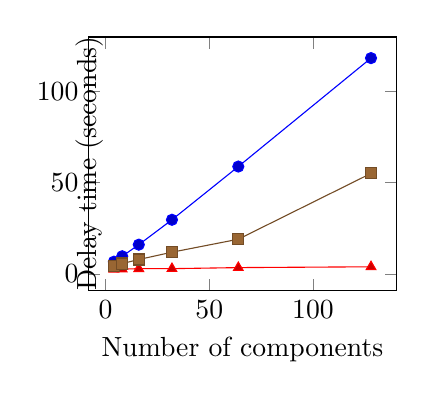
\begin{tikzpicture}
 \begin{axis}[
 	ylabel={Delay time (seconds)},
 	y label style={at={(0.08, 0.5)}},
 	xlabel={Number of components},width = 5.5cm,
 	height = 4.8cm]

 \addplot+[mark=*] coordinates
 	{(4,6.614953125) (8,9.60012962962963) (16,15.9376486486486) (32,29.564) (64,58.7045) (128,118.061571428571)};
 	
 \addplot+[mark=triangle*] coordinates
 	{(4,2.46368292682927) (8,2.56517142857143) (16,2.79086206896552) (32,2.81322222222222) (64,3.3868064516129) (128,3.83251724137931)};
 	
 \addplot+[mark=square*] coordinates
	 	{(4,4.31777777777778) (8,5.59077777777778) (16,7.81511538461538) (32,11.8165)  (64,18.9216363636364) (128,54.9538)};

 \end{axis}
 \end{tikzpicture}
 \caption{Delay time to detect fault with a\newline component size of 115 classes.\label{fig:delay-time-115}}
\end{minipage}
 % 4 classes
 \begin{minipage}[t]{0.45\linewidth}
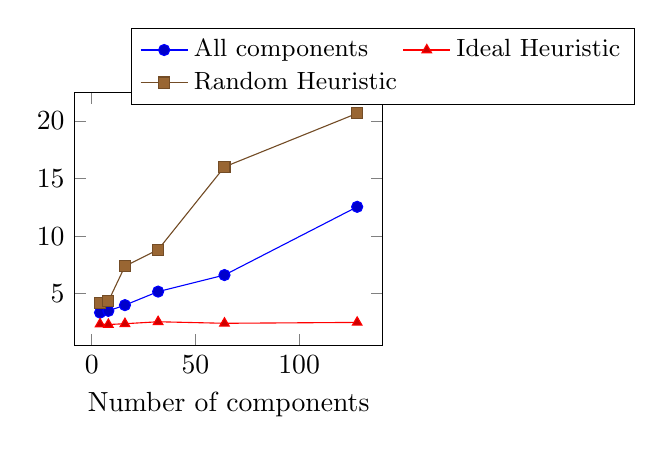
\begin{tikzpicture}
 \begin{axis}[
 	every axis legend/.append style={nodes={right}},
 	legend columns=2, 
 	legend style={at={(1.0,0.95)},
 	anchor=south,legend columns=1, font=\small},
 	xlabel={Number of components},width = 5.5cm,
 	height = 4.8cm]

 \addplot+[mark=*] coordinates
 	{(4,3.36101408450704) (8,3.51326153846154) (16,4.01246031746032) (32,5.18675) (64,6.62437704918033) (128,12.5490980392157)};
 	
 \addplot+[mark=triangle*] coordinates
 	{(4,2.3682619047619) (8,2.32882926829268) (16,2.39802777777778) (32,2.568) (64,2.43528571428571) (128,2.51225806451613)};
 	
 \addplot+[mark=square*] coordinates
	 	{(4,4.18407692307692) (8,4.35309090909091) (16,7.392) (32,8.82909090909091)  (64,16.017125) (128,20.6681428571429)};

	\legend{All components, Ideal Heuristic, Random Heuristic}
 \end{axis}
 \end{tikzpicture}
%\caption{4 classes}
 \caption{Delay time to detect fault with a\newline component size of four classes.\label{fig:delay-time-4}}
 \end{minipage}
\hspace{1cm}
\end{figure*}

 \begin{figure*}
 \centering
 % 115 classes
 \begin{minipage}[t]{0.45\linewidth}
 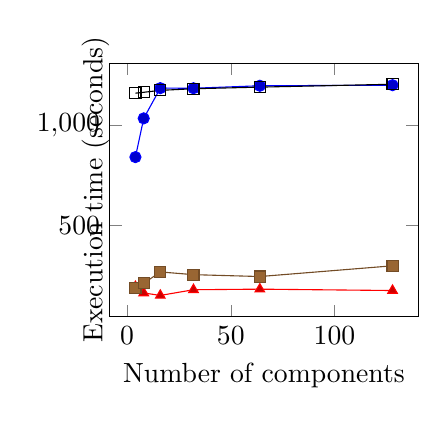
\begin{tikzpicture}
 \begin{axis}[
 	ylabel={Execution time (seconds)},
 	y label style={at={(0.03, 0.5)}},
 	xlabel={Number of components},width = 5.5cm,
 	height = 4.8cm]

 \addplot+[mark=*] coordinates
 	{(4,842.274) (8,1035.734) (16,1186.657) (32,1186.140) (64,1198.539) (128,1201.415)};
 	
 \addplot+[mark=triangle*] coordinates
 	{(4,195.609) (8,163.964) (16,151.637) (32,180.026) (64,182.962) (128,176.101)};
 	
 \addplot+[mark=square*] coordinates
	 	{(4,186.798) (8,211.913) (16,268.908) (32,255.329)  (64,245.976) (128,299.516)};
	 	
 \addplot+[mark=square] coordinates
	 	{(4,1161.593) (8,1165.910) (16,1175.643) (32,1183.620)  (64,1191.749) (128,1206.128)};
 \end{axis}
 \end{tikzpicture}
 \caption{Execution time of main\newline task with a component size\newline of 115 classes.\label{fig:execution-time-many-115}}
\end{minipage}
 % 4 classes
 \begin{minipage}[t]{0.45\linewidth}
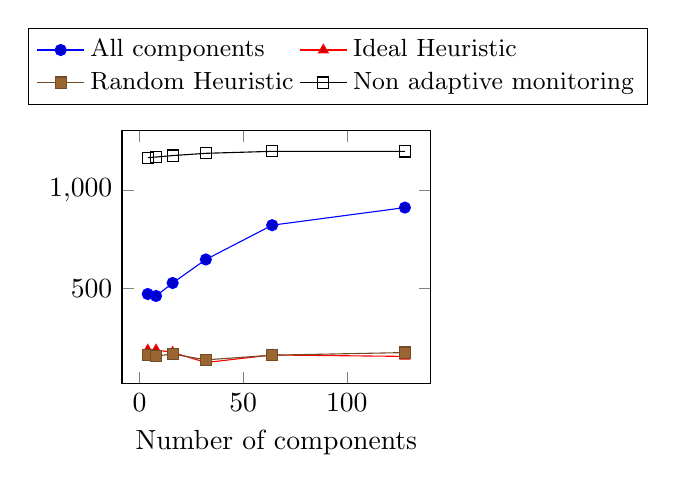
\begin{tikzpicture}
 \begin{axis}[
 	every axis legend/.append style={nodes={right}},
 	legend columns=2,
 	legend style={at={(0.7,1.1)},
 	anchor=south,legend columns=1, font=\small},
 	xlabel={Number of components},width = 5.5cm,
 	height = 4.8cm]

\addplot+[mark=*] coordinates
 	{(4,471.532) (8,461.274) (16,527.667) (32,647.634) (64,822.767) (128,912.634)};
 	
 \addplot+[mark=triangle*] coordinates
 	{(4,185.003) (8,185.533) (16,173.457) (32,121.551) (64,160.201) (128,152.802)};
 	
 \addplot+[mark=square*] coordinates
	 	{(4,161.985) (8,154.983) (16,164.704) (32,135.131)  (64,159.032) (128,172.392)};
	 	
 \addplot+[mark=square] coordinates
	 	{(4,1167.814) (8,1170.811) (16,1178.219) (32,1189.748)  (64,1199.834) (128,1199.453)};

	\legend{All components, Ideal Heuristic, Random Heuristic, Non adaptive monitoring}
 \end{axis}
 \end{tikzpicture}
 \caption{Execution time of main\newline task with a component size\newline of four classes.\label{fig:execution-time-many-4}}
 \end{minipage}
\hspace{1.5cm}
\end{figure*}


\subsubsection{Impact of the application size}
%\paragraph{Impact of the application size}
Figures \ref{fig:delay-time-4} and \ref{fig:execution-time-many-4} show the size of the application has an impact on the delay to detect faulty components, and also on the monitoring overhead.
We also calculated the time needed to find the faulty component with the \emph{All components} mode after its initialization (the time needed to switch from \emph{Global monitoring}).
This time is around 2 seconds no matter the size of the application.
That is the reason the switch from \emph{Global monitoring} to \emph{All components} has such a large effect on overhead.

These figures also show that using \emph{Localized monitoring} instead of \emph{All components} when switching from \emph{Global monitoring} helps reduce the impact of the application's size by reducing the number of components to monitor and the number of classes to instrument.
However, we also see that using a sub-optimal heuristic may have negatively impacted the delay to detect faulty components.
This can be explained by the multiple switches that the Random heuristic may often require to locate the faulty component.

\subsubsection{Impact of the component size}
%and \ref{fig:execution-time-many-115}, \ref{fig:execution-time-many-4}
In Figures \ref{fig:delay-time-115} and \ref{fig:delay-time-4} we can observe that the component size greatly impact the performance and the delay for ScapeGoat to find the faulty component. 
Similar to the explanation for the application's size, component size impacts the switch from \emph{Global monitoring} to \emph{Localized monitoring}, because of the class reloading and instrumentation.
A good heuristic drastically reduces the number of transitions; thus, it has a huge impact on the delay. 
When the components size increase, the choice of a good heuristics becomes even more important, because the cost of dynamic monitoring probes injection increase with the size of the components.
\section{Scapegoat to spot faulty components in a scalable diverse web application}\label{sec:WebStudy}
In this section, we present another application that benefits from the Scapegoat approach.
Although the general goal of spotting components that behave abnormally regarding resource consumption remains the same, with this use case we highlight the possibility of using Scapegoat 
%on a real application 
%and a specific usage of Scapegoat 
to automatically find buggy components on a scalable modular web application.
The section \ref{MdMS} presents an introduction to the application use case, while the remainder of the section deals with the experimental setup and the results.


\subsection{Use case presentation}\label{MdMS}
We are applying the Scapegoat approach to check resource consumption contracts on a web application called MdMS.\footnote{\url{https://github.com/maxleiko/mdms-ringojs}}
This application offers a web Content Management System based on the Markdown language for editing posts. 
MdMS uses a typical architecture (as shown in Figure \ref{fig:webapp}) for scalable web applications: a load-balancer connected to a set of workers (called MdMS Sosie in Figure \ref{fig:webapp}), which are themselves connected to a distributed database to retrieve the application specific content.
The worker layer of this application can be duplicated across various machines to support a growing number of clients.
The web application is currently online\footnote{\url{http://cloud.diversify-project.eu/}}. 

\begin{figure*}[!bt]
	\centering
	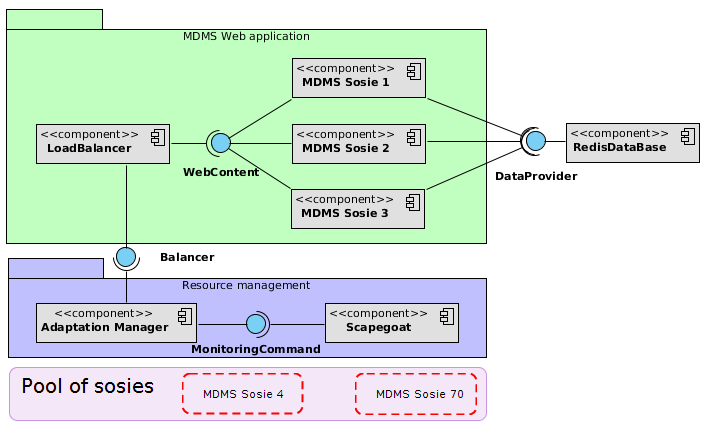
\includegraphics[scale=0.45]{./chapter5/figures/webapp2}
	\caption{\label{fig:webapp}Architecture of MdMS along with Scapegoat and additional components to adapt the system.}
\end{figure*}

The main characteristic of MdMS is that workers are not pure clones but diverse implementations of the MdMS server stack~\cite{alliermulti}.
This proactive diversification of MdMS targets safety~\cite{avizienis85} and security~\cite{Forrest97} purposes.
In particular, we have used a recent technique for the automatic synthesis of \textit{sosie} programs~\cite{baudry2014tailored} in order to automatically diversify the workers. 
A \textit{sosie} is a variant of a program that exhibits the same functionality (passes the same test suite) and a diverse computation (different control or data flow). 
\textit{Sosie} synthesis is based on the transformation of the original program through statement deletion, addition or replacement.
%The MdMS application is leveraging this diversified set of workers in order to reach the scalability property while icluding diversity in the software layer to prevent the so-called BOBE (Blow Once, Blow Everywhere) attacks~\cite{alliermulti}.

While the construction of \textit{sosies} focuses on preserving functional correctness, it ignores all the non-functional aspects of the program.
Consequently, a \textit{sosie} offers no guarantee regarding its resource consumption and may contain memory leaks or other overhead on resource consumption that can significantly impact the performance of MdMS.

In this experiment, we use Scapegoat to monitor the resource consumption of the various \textit{sosies} of the MdMS workers.
This technique enables us to identify \textit{sosies} in a production environment that do not behave according to the resource consumption contracts, allowing the system to remove these workers and use other \textit{sosies}.
Our goal in this experiment is to answer the following question:

\begin{itemize}
 \item Does Scapegoat correctly identify the faulty components in a system which includes many variants of the same component?   
\end{itemize}

\subsection{Experimental setup}

We devised this experiment as a scenario where many clients interact with the web application at the same time by adding and removing articles.
The stress produced by these requests increases the resource consumption on the server side which is running on top of Kevoree components.
Figure~\ref{fig:webapp} depicts the server side's configuration.
Since MdMS is a web application developed on top of RingoJS~\footnote{\url{https://github.com/ringo/ringojs}}, a JavaScript runtime written in Java, our \textit{sosies} include the RingoJS framework and the application that has been wrapped into Kevoree components.

In this experiment, we deploy many of these components as back-end servers of the web application and we use Scapegoat to monitor the consumption of each server.
Their contracts regarding resource consumption were built using the mechanism described in section \ref{sec:measurement_metodology} but with the original MdMS worker as a reference component.
The application also contains a component acting as a front-end that evenly distributes the requests among back-end servers.
This load balancer implements a plain round robin policy.
%There is an additional component running on the platform, it is in charge of adapting the system.
%This component reacts to events produced by Scapegoat and modifies the deployed system following the Models@run.time paradigm.

To produce a realistic load on the web server we have recorded a set of standard activities on the MdMS web site using Selenium~\footnote{\url{http://www.seleniumhq.org/}}.
We then use the Selenium facilities to replay these activities many times in parallel to provide the required work load on the server.
% of resource consumption, we generate many accesses to the system.
%We use Selenium~\footnote{http://www.seleniumhq.org/} to accomplish this purpose since MdMS is a web application.
Our experimental settings feature 120 clients which are scheduled by a pool of 7 concurrent Selenium workers.
Each client adds 10 articles to the database through the Website GUI, which represents 16 requests per article, for a total of 19200 requests to the MdMS workers sent through the load balancer.
In this experiment, the Selenium workers are executed on the same physical device as the web server, with the same testing platform described in section~\ref{sec:measurement_metodology}.

The experiment is configured as follows.
Using the diversification technique described in~\cite{baudry2014tailored}, we synthesized 20 \textit{sosies} of the MdMS workers.
These \textit{sosies} are used to execute the application with a varying number of back-ends (from 4 to 10).
One particular \textit{sosie} has been modified by hand to ensure that it violates the original component's contract.
We execute all the described components as well as the Scapegoat components on a single instance of Kevoree.

\subsection{Experimentation results}

Figure~\ref{fig:execution-time-web-app} shows the time required on the server side to reply to all the requests sent by Selenium.
Although the values might look surprisingly high at first, they are in fact the result of a heavily loaded system.
Selenium is actually rendering a couple of web pages for each added article; hence at least 2400 pages are rendered.
Moreover, both clients and servers are sharing resources because they run on the same physical device.
%Another point to highlight is that the time needed to execute all these requests remains stable when no monitoring is used and only changes abruptly when deploying ten \textit{sosies}.
%The execution times remain stable when monitoring is not activated, which is expected because the number of requests does not change between experiments, the load balancer distributes these requests evenly, and we are using the same physical device to execute all back-end servers.
%The stability of the executions when monitoring is not activated is expected because the number of requests does not change between experiments, the load balancer distributes these requests evenly, and we are using the same physical device to execute all back-end servers.
This leads to very stable execution times when monitoring is not activated because the number of requests does not change between experiments, the load balancer distributes these requests evenly, and we are using the same physical device to execute all back-end servers.
%\todo{Please, read below the explanation for: Why the execution time decreases?}
In the \textit{local monitoring} series, the global time to execute decreases until reaching 9 \textit{sosies}.
Although counterintuitive, it is caused by the effect of having \textit{localized monitoring} and \textit{load balancing} at the same time.
For instance, when four \textit{sosies} are used, the monitoring probes are periodically injected into one component out of four, hence roughly a quarter of the requests are handled by a slower \textit{sosie}.
However, with eight components the slow execution path is only taken by around 12.5\% of the requests.
The overhead of \textit{Localized monitoring} when ten \textit{sosies} are deployed increases because the physical machine reaches its limit and begins thrashing.
As a consequence, low-level interactions with the hardware (e.g. cache misses), the operating system and the JVM slow down the execution.
On average, the overhead due to monitoring with both instruction instrumentation and memory instrumentation is 1.59, which is lower than the values shown in section~\ref{sec:OverheadFullMonitoring} for full monitoring despite only one of the instrumentation mechanisms being enabled in those experiments.
The values in this section are better even if we are monitoring both resources because we are using the adaptive approach.
   

\begin{figure*}
 \centering
 \begin{minipage}[t]{0.43\linewidth}
 \centering
 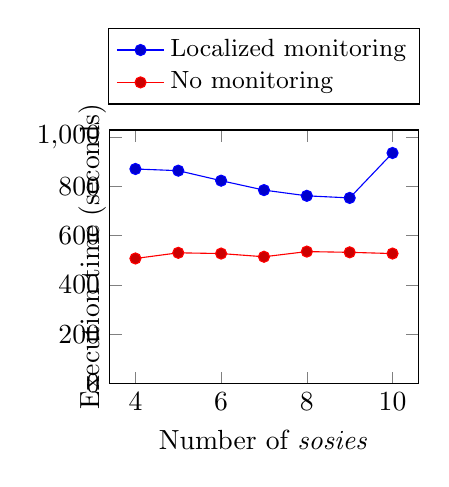
\begin{tikzpicture}
  \begin{axis}[
  	ylabel={Execution time (seconds)},
  	y label style={at={(0.02, 0.5)}},
  	legend style={at={(0.5,1.1)},
  	 	 	anchor=south,legend columns=1, font=\small},
  	ymin=0,
  	every axis legend/.append style={nodes={right}},
  	xlabel={Number of \textit{sosies}},width = 5.5cm,
  	height = 4.8cm]
 
  \addplot+[mark=*] coordinates
  	{(4, 870.375) (5, 863.5) (6, 822.875) (7, 784.625) (8, 761.375) (9, 752.875) (10, 935.3)};

\addplot+[mark=*] coordinates
  	{(4, 507) (5, 530) (6, 527) (7, 514) (8, 535) (9, 532) (10, 527)};
  	
  	\legend{Localized monitoring, No monitoring}
  	
  \end{axis}
  \end{tikzpicture}
  \caption{Time to obtain the reply to all requests.\label{fig:execution-time-web-app}}
  \end{minipage}
  \hspace{0.1\linewidth}
 \begin{minipage}[t]{0.43\linewidth}
 \centering
 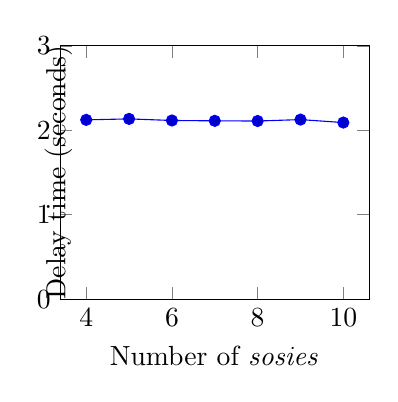
\begin{tikzpicture}
 \begin{axis}[
 	ylabel={Delay time (seconds)},
 	y label style={at={(0.07, 0.5)}}, 	
 	ymin=0,ymax=3,
 	xlabel={Number of \textit{sosies}},width = 5.5cm,
 	height = 4.8cm]

 \addplot+[mark=*] coordinates
 	{(4,2.1235) (5, 2.1348) (6,2.11605) (7,2.1119) (8, 2.1097) (9, 2.12654) (10, 2.09139)};
 	
 \end{axis}
 \end{tikzpicture}
 \caption{Average delay time to detect a faulty \textit{sosie}.\label{fig:delay-time-web-app}}
\end{minipage}

\hspace{1cm}
\end{figure*}


In these experiments, we evaluate the accuracy of the output and its quality in terms of the time needed to find the faulty component.
Scapegoat always spots the correct \textit{sosie}.
It does so because it is an iterative process that continues until finding the faulty component.
In addition, Scapegoat does not output false positives during these experiments.
The delay to detect faulty components is shown in Figure~\ref{fig:delay-time-web-app}.
In this case, the values remain close to 2 seconds no matter the number of \textit{sosies} used nor the execution time.
This behavior is consistent with the experiments in section~\ref{sec:evaluation} because we are also using a good heuristic for the use case.
It shows that Scapegoat can spot faulty components with an acceptable delay in a real application.

\subsection{Discussion of the use case}
This use case shows that Scapegoat is able to provide useful information in real applications.
It also highlights how the framework can help select software variants at runtime in the context of software diversity.
Or, more generally, in the field of software oriented architectures where many stakeholders may provide the same services, Scapegoat can help to choose services.
Moreover, this use case leads to a distributed usage of Scapegoat, where the policies for admission control and resource consumption monitoring can be coordinated among distributed devices.

Finally, in systems where there are many variants of the same component or service, Scapegoat provides essential information to drive application reconfiguration.
For example, the adaptation component in Figure~\ref{fig:webapp} may use Scapegoat's faulty component selection to replace a faulty \textit{sosie} or to modify the scheduling policy in the load balancer.






%\section{Related work}\label{sec:related}

The Scapegoat framework is related to component monitoring, Models@run.time, component isolation and component performance prediction approaches.

Performance and resource-consumption prediction approaches are complementary to the Scapegoat framework because they can assist in better specifying the component contracts.
Some approaches require developers to provide extensive per-component metadata at design-time in order to calculate the application's overall performance or resource consumption \cite{Becker:2007:MPP:1216993.1217006,Jonge03scenario-basedprediction}.
Prediction approaches have been achieved by using combinations of design-time and runtime analyses \cite{autili2012hybrid}.
However, although many approaches to performance prediction have been proposed, none of them have obtained widespread use \cite{Koziolek:2006:QDD:2171366.2171393}.

%In \cite{Ghezzi2009}, the authors propose using performance models based on Queuing Networks to cope with the problem of architectural reasoning.
%The authors keep Models@run.time to enable re-estimation of model parameters based on the behavior of the running system and they present a mechanism to update the parameters when usage profiles change.
%The authors target the same problem we are dealing with, although we are not facing the prediction of behavior.

KAMI \cite{Ghezzi2009} builds performance models at design-time but uses and continually refines them at runtime.
By collecting runtime data, they are able to build performance and resource consumption models that reflect real usage.
They are able to adapt the application according to changes in components' behavior, but they do not use nor propose an adaptive monitoring system to minimize overhead.

%\todo{For Walter: Review this paragraph}
State of the art monitoring systems \cite{FrenotS04,KregerHaroldWilliamson03,Binder200645} extract steady data-flows of system parameters, such as, the time spent executing a component, the amount of I/O and memory used, and the number of calls to a component.
The overhead that these monitoring systems introduce into applications is high, which makes it unlikely for them to be used in production systems.
Maurel et al. \cite{Maurel:2012:AME:2304736.2304763} propose an adaptive monitoring framework for the OSGi platform.
Similar to our approach, they propose a global monitoring system that changes to a localized monitoring system when a problem is detected.
However, their work is focused on CPU usage and does not consider other resources, such as memory or I/O.
Exploring the Java heap to obtain useful information about resource consumption has been proposed in~\cite{Price:2003:GCM:829515.830545, Geoffray5270296}.
As in our work, they account objects to the resource principal being explored (in their case to OSGi bundles) the first time an object is reached.
Their solutions modify the garbage collector in order to reduce overhead, but this causes resource accounting to be tied to, and performed on, each collection cycle.
%but it means that the accounting step is performed on each collection cycle.
In contrast, our approach can be executed on demand, albeit at the cost of further passes over the heap.
%although our accounting step requires further passes over the heap, we can precisely specify when to execute it.

Gama and Donsez \cite{Gama:2010:SCS:2176905.2176915} propose using virtual machines in separate processes or using MVM isolates \cite{czajkowski2012multitasking} to manage trusted and untrusted components.
After an evaluation period, untrusted components can be moved to the trusted JVM if no problems are detected.
This allows the main application to depend on potentially faulty components without risking severe crashes.
We can also cite Microsoft technologies such as COM (Component Object Model) components which can be either loaded in the client application process or provided in an isolated process \cite{lowy2001and}.
In addition to process virtualization, some operating systems also propose user-space virtualization, which isolates not only the processes but also the memory, the network interface and the file system. Examples of these approaches are Jails\footnote{\url{http://www.freebsd.org/doc/handbook/jails.html}} for BSD, LXC\footnote{\url{http://lxc.sourceforge.net/}} and CGroups for Linux, and lmctfy\footnote{\url{https://github.com/google/lmctfy}}.
All of these approaches have the drawback of limiting code and instance sharing and introduce additional overhead in cross-boundary component interactions.
Furthermore, depending on the complexity of the approach, there is also overhead in having to manage multiple processes.

\section{Conclusions}\label{sec:conclusion}
In this chapter we presented Scapegoat, an adaptive monitoring framework to perform lightweight yet efficient monitoring of Component-Based Systems.
In Scapegoat, each component is augmented with a contract that specifies its resource usage, such as peak CPU and memory consumption.
Scapegoat uses a global monitoring mode that has low overhead on the system, and an on-demand fine-grained localized monitoring mode that performs extensive checking of the components' contracts.
The system switches from the global monitoring mode to the localized monitoring mode whenever a problem is detected at the global level in order to identify the faulty component.
Furthermore, we proposed a heuristic that leverages information produced by the Models@run.time approach to quickly predict the faulty components. 

Scapegoat has been implemented on top of the Kevoree component framework which uses the Models@run.time approach to tame the complexity of distributed dynamic adaptations.
The evaluation of Scapegoat shows that the monitoring system's overhead is reduced by up to 92.98\% in comparison with state-of-the-art full monitoring systems. 
The evaluation also presents the benefits of using a heuristic to predict the faulty component.
In the second part of the evaluation, we highlighted the benefit of Scapegoat on a classical web server architecture to dynamically determine faulty components.
This second example also exposes the capacity of Scapegoat to be applied to different application domains and confirms its relatively low overhead on the running system.
Scapegoat contributes to the state of the art by providing a monitoring framework which adapts its overhead depending on current execution conditions and leverages the architectural information provided by Models@run.time to drive the search for the faulty component.

The approach proposed in this chapter contributes to answer two research questions that were presented in the introduction of this thesis (see Section \ref{sec:intro-challenges}).
In particular, it answers \textit{RQ1} (\textit{How can we provide portable and efficient support for resource consumption monitoring?}) by describing a monitoring framework that produces low performance overhead and is fully portable.
Likewise, our proposal partially answers \textit{RQ3} (\textit{How can we leverage the knowledge about the architecture of applications to drive
a mechanism for resource management?}) by using knowledge about the structure of applications to drive the behavior of the framework.

